\documentclass[12pt,legalpaper]{report}
\usepackage[utf8x]{inputenc}
\usepackage{ucs}
\usepackage[spanish]{babel}
\usepackage{amsmath}
\usepackage{amsfonts}
\usepackage{amssymb}
\usepackage{graphicx}
\usepackage{moreverb} 
\usepackage{hyperref}
\usepackage{colortbl}
\usepackage[doublespacing]{setspace}
\usepackage[left=4cm,top=4cm,right=3cm,bottom=3cm]{geometry}
\pagestyle{headings}
\hypersetup{colorlinks=false, draft = true}
\usepackage{appendix}
\usepackage[T1]{fontenc}
\setcounter{secnumdepth}{6}
\setcounter{tocdepth}{6}
\renewcommand{\appendixname}{Apéndice}
\renewcommand{\appendixpagename}{Apéndices}
\renewcommand{\appendixtocname}{Apéndices}
%para funcionamiento de listings
\usepackage{times}
\usepackage{color}
\definecolor{gray97}{gray}{.97}
\definecolor{gray75}{gray}{.75}
\definecolor{gray45}{gray}{.45}
\usepackage{listings}
\lstset{ 
	frame=Ltb,
	framerule=0pt,
	aboveskip=0.5cm,
	framextopmargin=3pt,
	framexbottommargin=3pt,
	framexleftmargin=0.4cm,
	framesep=0pt,
	rulesep=.4pt,
	backgroundcolor=\color{gray97},
	rulesepcolor=\color{black},
	%
	stringstyle=\ttfamily,
	showstringspaces = false,
	basicstyle=\small\ttfamily,
	commentstyle=\color{gray45},
	keywordstyle=\bfseries,
	%
	numbers=left,
	numbersep=15pt,
	numberstyle=\tiny,
	numberfirstline = false,
	breaklines=true,
}

% minimizar fragmentado de listados
%\lstrenewenvironment{listing}[1][]
%   {\lstset{#1}\pagebreak[0]}{\pagebreak[0]}
 
\lstdefinestyle{consola}
{
	basicstyle=\scriptsize\bf\ttfamily,
	backgroundcolor=\color{gray75},
}
 
\lstdefinestyle{python}
{
	language=python
}


\begin{document}
%\title{}
%\author{Milton Inostroza Aguilera}
%\date{}
%\clearpage
%\maketitle
\thispagestyle{empty}
\begin{singlespace}
\begin{figure}[hpb]
	\centering
	
\includegraphics[scale=0.15]{images/logo.eps}
\end{figure}
\begin{center}

\vspace{-0.7cm}
DEPARTAMENTO DE INGENIERIA\\[4cm]

\begin{doublespace}
{\textbf ANALISIS, DISEÑO E IMPLEMENTACION DE pyTOD, UN PROTOTIPO EXPERIMENTAL PARA REALIZAR DEPURACION OMNISCIENTE A SCRIPTS ESCRITOS EN EL LENGUAJE DE PROGRAMACION PYTHON}\\[3cm]
\end{doublespace}
{\small ACTIVIDAD DE TITULACION PRESENTADA PARA OPTAR A:\\
GRADO ACADEMICO DE LICENCIADO EN CIENCIAS DE LA INGENIERIA\\
TITULO DE INGENIERO CIVIL EN COMPUTACION E INFORMATICA}\\[3cm]

\begin{table}[!h]
\begin{tabular}{r l}
{\small ALUMNO :} & {\small MILTON INOSTROZA AGUILERA}\\
\\
{\small PROFESOR GUIA :} & {\small DAVID CONTRERAS AGUILAR}\\
\\
{\small PROFESOR CORRECTOR :} & {\small WILSON CASTILLO ROJAS}\\
\end{tabular}
\end{table}
\vspace{5cm}
IQUIQUE - CHILE\\
2008
\end{center}
\end{singlespace}

\begin{abstract}

La depuración es la mayor tarea del proceso de construcción de programas de un software, considerándolo en términos de tiempo y costo. Desafortunadamente los depuradores en muchos ambientes de desarrollo de programas de un software sólo entregan una asistencia mínima contribuyendo a que la depuración sea algo tedioso y una tarea que consume mucho tiempo.

Existen dos métodos tradicionales para realizar depuración de programas de un software: 

\begin{enumerate}
	\item log-based, basado en mensaje, y
	\item break point-based, basado en punto de quiebre.
\end{enumerate}
	
La primera propuesta consiste en ir insertando registros de declaraciones dentro del código fuente, en el orden que se produce una huella ad-hoc durante la ejecución del programa. Esta técnica expone la historia actual de ejecución pero: 

\begin{itemize}
	\item Requiere grandes modificaciones del código fuente.
	\item Esta técnica no es escalar, debido a que el análisis manual de grandes huellas es complicado. 
\end{itemize}

El segundo método consiste en ejecutar el programa bajo un depurador dedicado cuando el programador permita pausar la ejecución en un punto determinado del software, examinando el contenido de la memoria, y pudiendo continuar la ejecución paso a paso. A pesar de lo anterior, breakpoint-based debugging es limitado: cuando la ejecución es pausada, la información sobre el estado y actividad anterior del programa es limitada por la introspección\footnotemark[1] de la pila\footnotemark[2] de llamada actual.

\footnotetext[1]{Instrospección: Capacidad de un programa de razonar sobre su propia estructura}
\footnotetext[2]{Pila: Estructura de datos de tipo LIFO que permite almacenar y recuperar datos}


Aunque los dos métodos anteriormente señalados han sido utilizados ampliamente existe una tercera propuesta llamada depuración omnisciente, también conocida como atrás-en-el-tiempo o después-de-la-muerte, superan todas las características de los métodos anteriores. Un depurador omnisciente registra los eventos que ocurren durante la ejecución del programa depurado y en seguida entrega al usuario un conveniente navegador por medio del cual obtiene la huella de ejecución.  Esta propuesta combina las ventajas de la depuración basada en log -- la actividad pasada no se pierde nunca -- y también la de depuración basada en break point -- fácil navegación, ejecución paso a paso e inspección completa de la pila de ejecución. Un depurador omnisciente puede simular la ejecución paso a paso hacia adelante y hacia atrás, y es posible construir inmediatamente preguntas/respuestas que podrían de una u otra forma exigir un esfuerzo significante al programador, como ¿en qué punto la variable \textit{x} fue asignada al valor \textit{y}? o ¿en qué estado estaba el objeto \textit{o} cuando se le pasó un argumento al método \textit{foo}?.

Es importante señalar que los depuradores omniscientes además de superar todas las características anteriormente señaladas poseen una característica única y es la de identificar la causa inicial de los bugs\footnotemark[3].

\footnotetext[3]{Bug: Defecto de software}

Existen varias implementaciones de los depuradores omniscientes, pero se basará el caso de estudio en TOD\footnotemark[4], un depurador omnisciente orientado a la huella de ejecución.  TOD depura sólo programas escritos en Java y para esto brinda cuatro características principales:

\footnotetext[4]{TOD: Trace-Oriented debugger, implementado en el lenguaje de programación Java}

\begin{enumerate}
         \item Stepping, ejecución paso a paso del programa a depurar.
         \item Estado de reconstitución.
         \item Reconstitución del control de flujo.
         \item Identificar la causa inicial de los bugs.
\end{enumerate}

El desafío que se plantea en este trabajo de título es diseñar un prototipo experimental llamado pyTOD que permita realizar depuración omnisciente a scripts escritos en un lenguaje de tipado dinámico llamado Python, basándose en el estudio, análisis y utilización de TOD.

\end{abstract}

\newpage
\tableofcontents
\newpage
\listoffigures
\newpage
\listoftables
\newpage

\chapter{Introducción}

El proceso de depuración de programas de un software se hace cada vez más necesario debido al crecimiento y evolución de los lenguajes de programación (cambios de paradigmas y características).  Es importante que el programador disponga de ambientes adecuados para que de una forma fácil, rápida e intuitiva pueda corregir los defectos del software.  Si el programador no cuenta con un ambiente adecuado para poder inspeccionar los programas de su software y corregir ciertas anomalías el costo y tiempo del desarrollo de software aumenta dramáticamente \cite{cost}. En muchos casos los programas de un software desarrollado no son expuestos a pruebas exhaustivas para conocer su verdadero comportamiento en diversos ambientes, debido a lo costoso de esto, lo que conlleva a tener comportamientos inesperados en la fase de producción de estos.

El proceso anterior se define como la manera de identificar y eliminar errores dentro de un programa perteneciente a un software y sigue siendo, hoy en día a pesar del avance de la tecnología, en buena medida una actividad manual.  Actividad que desafía la paciencia, imaginación e intuición de los programadores.  En muchos casos los programadores deben incluir en el código fuente instrucciones auxiliares que permitan el seguimiento de la ejecución del programa, presentando los valores de variables, direcciones de memoria o lo que les sea necesario.

Es deseable que una herramienta de depuración de programas de un software evite que los programadores tengan que introducir lineas adicionales en sus programas para intentar saber el comportamiento de ciertos componentes de su software.

Es de esta forma como la industria del software ha planteado diversas soluciones, las cuales mitigan el pesado proceso de depuración de programas de un software.  Las soluciones mayormente utilizadas son los depuradores basados en logs y basados en puntos de quiebre, relegando de forma inexplicable la solución de los depuradores omniscientes.  Es en este punto donde nacen preguntas fundamentales tales como ¿conociendo las bondades de los depuradores omniscientes por qué no son ampliamente utilizados?, ¿a los programadores sólo les basta con los depuradores break-point based y log-based?, ¿cuáles son las desventajas que hace impracticable implementar un depurador omnisciente?, ¿no es necesario para el programador conocer la principal causa del defecto de software?.

Enfocándose en la solución de depuración omnisciente, no basta con sólo almacenar la historia del programa depurado, si no que se debe contar con un almacen de datos adecuado que sea escalable y eficiente para guardar esta enorme cantidad de información.  Además de esto, un depurado omnisciente debe implementar una interfaz que responda en un tiempo aceptable todas las peticiones que el programador le solicite.

Es por lo anterior que se ha seleccionado como caso de estudio TOD (Trace-oriented Debugger) \cite{tod} un depurador omnisciente con almacenamiento escalable.  Su interfaz gráfica responde rápidamente a las peticiones del programador y la sobre carga que produce en el ambiente en el cual se ejecuta es menor que otras implementaciones existentes sobre este concepto.

De este modo, este trabajo de memoria se centra en la implementación de un prototipo experimental, el cual realice depuración omnisciente a scripts escrito en el lenguaje de programación Python, utilizando como base de estudio e implementación TOD, un depurador omnisciente escrito en el lenguaje de programación Java.

\chapter{Propósito general}

Como concepto general se dice que software es el conjunto de programas de cómputo, procedimientos, reglas, documentación y datos asociados que forman parte de las operaciones de un sistema de computación. \cite{ieee}

La ingeniería de software plantea que existen tres grandes procesos para desarrollar software, que se detallan en orden cronológico:
\begin{enumerate}
	\item Análisis de sistema
	\item Diseño de sistema
	\item Codificación de software.
\end{enumerate}

En especial nos centraremos en el último proceso en el cual se realizan las tareas que comúnmente se conocen como programación; que consiste, escencialmente, en llevar a código fuente, en el lenguaje de programación elejido, todo lo diseñado en la fase anterior. Esta tarea la realiza el programador, siguiendo por completo los lineamientos impuestos en el diseño y en consideración siempre a los requisitos funcionales y no funcionales (ERS) especificados en la primera etapa.

Es común pensar que la etapa de programación o codificación (algunos la llaman implementación) es la que consume la mayor parte del trabajo de desarrollo del software; sin embargo, esto puede ser relativo (y generalmente aplicable a sistemas de pequeños) ya que las etapas previas son cruciales, críticas y pueden llevar bastante más tiempo. Se suele hacer estimaciones de un 30\% del tiempo total consumido en la programación, pero esta cifra no es consistente ya que depende en gran medida de las características del sistema, su criticidad y el lenguaje de programación elegido. En tanto menor es el nivel del lenguaje mayor será el tiempo de programación requerido, así por ejemplo se tardaría más tiempo en codificar un algoritmo en ensamblador que el mismo programado en lenguaje C.

Durante la fase de programación, el código puede adoptar varios estados, dependiendo de la forma de trabajo y del lenguaje elegido.  Para introducir conceptos fundamentales en este tema de memoria, es importante precisar lo siguiente:

\begin{description}

    \item[Código fuente] Es el escrito directamente por los programadores en editores de texto, lo cual genera el programa. Contiene el conjunto de instrucciones codificadas en algún lenguaje de alto nivel. Puede estar distribuido en paquetes, procedimientos, librerías fuente, etc.

    \item[Código objeto] Es el código binario o intermedio resultante de procesar con un compilador el código fuente. Consiste en una traducción completa y de una sola vez de éste último. El código objeto no es inteligible por el ser humano (normalmente es formato binario) pero tampoco es directamente ejecutable por la computadora. Se trata de una representación intermedia entre el código fuente y el código ejecutable, a la espera de un enlace final con las rutinas de librería y entre procedimientos.

	\begin{itemize}
		\item El código objeto no existe si el programador trabaja con un lenguaje a modo de intérprete puro, en este caso el mismo intérprete se encarga de traducir y ejecutar línea por línea el código fuente (de acuerdo al flujo del programa), en tiempo de ejecución. En este caso tampoco existe él o los archivos de código ejecutable. Una desventaja de esta modalidad es que la ejecución del programa o sistema es un poco más lenta que si se hiciera con un intérprete intermedio, y bastante más lenta que si existe el o los archivos de código ejecutable. Es decir no favorece el rendimiento en velocidad de ejecución. Pero una gran ventaja de la modalidad intérprete puro, es que el esta forma de trabajo facilita enormemente la tarea de depuración del código fuente (frente a la alternativa de hacerlo con un compilador puro). Frecuentemente se suele usar una forma mixta de trabajo (si el lenguaje de programación elejido lo permite), es decir inicialmente trabajar a modo de intérprete puro, y una vez depurado el código fuente (liberado de errores) se utiliza un compilador del mismo lenguaje para obtener el código ejecutable completo, con lo cual se agiliza la depuración y la velocidad de ejecución se optimiza.
	\end{itemize}

	\item[Código ejecutable] Es el código binario resultado de enlazar uno o más fragmentos de código objeto con las rutinas y librerías necesarias. Constituye uno o más archivos binarios con un formato tal que el sistema operativo es capaz de cargarlo en la memoria RAM (eventualmente también parte en una memoria virtual), y proceder a su ejecución directa. Por lo anterior se dice que el código ejecutable es directamente "inteligible por la computadora". El código ejecutable, también conocido como código máquina, no existe si se programa con modalidad de "intérprete puro".

	\item[Compilador] Es un programa informático que traduce un programa escrito en un lenguaje de programación a otro lenguaje de programación, generando un programa equivalente que la máquina será capaz de interpretar. Usualmente el segundo lenguaje es código máquina, pero también puede ser simplemente texto. Este proceso de traducción se conoce como compilación.Un compilador es un programa que permite traducir el código fuente de un programa en lenguaje de alto nivel, a otro lenguaje de nivel inferior (típicamente lenguaje máquina). De esta manera un programador puede diseñar un programa en un lenguaje mucho más cercano a como piensa un ser humano, para luego compilarlo a un programa más manejable por una computadora.

	\item[Intérprete] Es un programa informático capaz de analizar y ejecutar otros programas, escritos en un lenguaje de alto nivel. Los intérpretes se diferencian de los compiladores en que mientras estos traducen un programa desde su descripción en un lenguaje de programación al código máquina del sistema destino, los primeros (los intérpretes) sólo realizan la traducción a medida que sea necesario, típicamente, instrucción por instrucción, y normalmente no guardan el resultado de dicha traducción.
	
\end{description}

Mientras se programa la aplicación, sistema, o software en general, se realizan también tareas de depuración, esto es la labor de ir liberando al código de los errores factibles de ser hallados en esta fase (de semántica, sintáctica y lógica). 

De acuerdo con Grace Murray Hopper, uno de los pioneros de la ciencia de la computación, la situación que dio origen al término depuración sucedió a principio de la década de los años 1950, los programadores de la Universidad de Harvard gastaron semanas en intentos infructuosos para encontrar el error en uno de sus programas. Finalmente, una investigación dentro de las computadoras reveló que un insecto había muerto ahí. Una vez removido el insecto, el programa funcionó correctamente. Desde entonces, el proceso de quitar errores de los programas ha sido llamado \textit{depuración}.

Pero, de acuerdo a Edsgar Dijkstra, otro pionero en las ciencias de la computación, el término es irresponsable. Depuración sugiere que el programador no tiene la culpa por el error. Esto es como si el insecto trepara dentro del código mientras el programador estaba mirando hacía otro lado.

Aunque el término tenga algunas dicidencias podemos decir que depuración es un proceso metódico, el cual encuentra y reduce el número de bug, o defectos, en un programa de computación, haciendo de esta forma que estos se comporten como es esperado.  La depuración tiende a ser dura cuando varios subsistemas, que contienen muchos programas, están estrechamentes acoplados, y cambios en uno pueden provocar bugs en otros.

La Depuración es, en general, una pesada y cansadora tarea.  La habilidad para depurar del programador es probablemente el mayor factor en la capacidad de resolver un problema, pero la dificultad de la depuración de software varía enormemente referente al lenguaje de programación utilizado y las herramientas disponibles, tal como los depuradores.  

Los depuradores son herramientas de software, las cuales habilitan al programar para monitorear la ejecución de un determinado programa, detenerlo, reactivarlo, poner puntos de quiebre, cambiar valores en memoria e incluso, en algunos casos, ir atrás en el tiempo.  El término depurador puede ser además relacionado con la persona quien hace la depuración.

Generalmente, los lenguajes de alto nivel, hacen la depuración fácil, porque ellos tienen características tales como manejo de excepciones que permiten manejar el comportamiento errático de una manera fácil.  En los lenguajes de nivel medio como C o bajo nivel tal como ensamblador, los bugs pueden causar silenciosos problemas tal como corrupción de memoria, y esto frecuentemente dificulta ver donde el problema principal ha ocurrido.  En estos casos, las herramientas de depuradores de memoria pueden ser útiles.

En determinadas situaciones, herramientas de software de propósito general que son lenguajes específicos pueden ser muy útiles.  Estas son llamadas herramientas de análisis estático.  Estas herramientas observan problemas conocidos que son muy específicos, algunos comunes y algunos extraños, dentro del código fuente.  Cada uno de estos son detectados por estas herramientas y raramente son detectados por el compilador o intérprete, por lo tanto ellos no son correctores sintácticos, si no más bien correctores semánticos.


	\section{Herramientas}

Un depurador es un software que es utilizado para probar y depurar otros programas.  Una técnica que permite gran utilidad en esto es la capacidad de suspender el programa depurado, cuando una condición específica es encontrada.

Cuando un programa lanza un error, el depurador muestra la posición en el código original donde se produjo dicho error, esto si es que es un depurador a nivel de código fuente, comunmente vistos en ambientes de desarrollos integrados.  Un lanzamiento de error sucede cuando el programa no puede manejar un comportamiento extraño o desconocido debido a un defecto de software (más conocido como Bug).  Por ejemplo, tal vez el programa intentó utilizar una instrucción no disponible en la versión actual de la CPU o intentó acceder a memoria no disponible o protegida.

Comúnmente, los depuradores además ofrecen prestaciones más sofisticadas como ejecutar un programa paso a paso (step by step), detener la ejecución (detener le ejecución del programa para examinar el estado actual) en algún tipo de evento mediante un punto de quiebre (breakpoint), y seguirle la pista a los valores de determinadas variables.  Algunos depuradores tienen la capacidad de modificar el estado del programa mientras este se ejecuta y así no solamente son meros expectadores de la ejecución de éste.

	\section{Proceso de depuración}

La depuración comienza tratando de reproducir un problema.  Esto puede ser una tarea no trivial, por ejemplo en el caso de procesos paralelos o algún problema inusual de software.  Además el ambiente específico del usuario y el uso de la historia puede hacer que sea dificil reproducir el problema.

Después de que el bug es reproducido, la entrada del programa necesita ser simplificada para hacer más fácil el proceso de depuración.  Por ejemplo, un bug en un compilador puede hacer que este falle cuando este analizando sintácticamente un programa fuente muy largo.  Tal simplificación puede ser realizada manualmente, utilizando un enfoque \textit{divide y vencerás}.  El programador intentará sacar algunas partes del caso original de prueba y verificar si el problema aún continúa.  Cuando se depura el problema en una interfaz gráfica, el programador tratará de saltarse alguna interacción desde la descripción original del problema y verificar si las acciones restantes son suficientes para que aparezca el bug.

Después de que el caso de prueba es suficientemente simplificado, el programador puede usar el depurado para examinar el estado del programa (valores de las variables, la pila de llamadas) e identificar el origen del problema.  De forma alternativa un rastreo puede ser utilizado.  En un caso sencillo el rastreo consiste sólo en algunas instrucciones de impresión, las cuales muestran el valor de las variables en determinados puntos del programa en ejecución.

La depuración remota es el proceso de depuración de un programa que está ejecutándose en un sistema diferente que el depurador.  Para comenzar la depuración remota, el depurador se conecta a un sistema remoto sobre una red de datos.  Una vez conectado, el depurador puede controlar la ejecución del programa  sobre un sistema remoto y recobrar la información sobre el estado de éste.

	\section{Objetivo general}

El objetivo general de este trabajo de memoria es:
\begin{itemize}
\item Construir un prototipo experimental llamado pyTOD para realizar depuración omnisciente a scripts escritos en el lenguaje de programación Python, utilizando como base de estudio TOD, un depurador omnisciente implementado en el lenguaje de programación Java.
\end{itemize}

    Esto implica brindar un ambiente de depuración que sea eficiente para el programador, además de entregar una herramienta básica para inspeccionar programas y poder encontrar las causas de los bugs.

	\section{Objetivos específicos}

Para lograr el éxito del objetivo general de este trabajo de título se han definido los siguientes objetivos específicos:

\begin{itemize}
\item[1.] \textit{Diseñar e Implementar un sistema que instrumente\footnotemark[1] el código Python de tal forma que envíe eventos a la base de datos de TOD.}
\end{itemize}
\footnotetext[1]{Agregar instrucciones al código para que realice determinadas tareas}

A través de la metodología de ensayo y error se implementará un capturador de huella de ejecución ad-hoc, que capturará todos los sucesos ocurridos en el programa objetivo escrito en Python, para luego enviarlos a la base de datos de TOD.


\begin{itemize}
\item[2.] \textit{Analizar la compatibilidad del modelo actual de huella de ejecución\footnotemark[2] de TOD con el lenguaje de programación Python.}
\end{itemize}

\footnotetext[2]{Secuencia ordenada de eventos heterogéneos de un programa computacional.}

Una vez que el capturador de huellas funcione parcialmente, se comenzará con el estudio de compatibilidad de huella de ejecución de TOD.  De ser necesario el modelo actual de huella de ejecución de TOD será modificado para conseguir compatibilidad con pyTOD.

\begin{itemize}
\item[3.] \textit{Diseñar e Implementar un protocolo de comunicación entre pyTOD (Python) y TOD (Java)}
\end{itemize}

Será necesario implementar un protocolo de comunicación el cual transporte la huella de ejecución creada en pyTOD hacía la base de datos de TOD.  Esto se realizará una vez que se haya analizado y modificado el modelo de huella de ejecución de TOD.

%\begin{itemize}
%\item[4.] \textit{Diseñar e Implementar una interfaz gráfica para el depurador pyTOD.}
%\end{itemize}

%De ser necesario se construirá una interfaz gráfica en la cual el usuario pueda interactuar con el programa depurado.  Para esto se debe evaluar si la actual interfaz gráfica de TOD sirve y es compatible.  De ser compatible realizando modificaciones se tomará esta opción como valida y se reutilizará este componente.

\begin{itemize}
\item[4.] \textit{Diseñar e Implementar un plugin para eclipse el cual permita conectar la interfaz gráfica del depurador con el ambiente de desarrollo.}
\end{itemize}

No basta con tener una interfaz gráfica independiente del ambiente de desarrollo del programador, es fundamental que la interfaz de usuario del depurador sea incorporado como plugin dentro del ambiente de desarrollo.  Para este caso se considerará como ambiente de desarrallo el IDE Eclipse\footnotemark[1].  Se utilizará el plugin de Python para Eclipse, PyDev como base de extensión para el nuevo plugin el cual permita al programador una interacción transparente entre el ambiente de desarrollo y el ambiente de depuración.

\footnotetext[1]{Entorno integrado de desarrollo de software}

\begin{itemize}
\item[5.] \textit{Aplicar pyTOD en un caso de prueba real.}
\end{itemize}

El resultado de éxito y contribución de este trabajo de título depende mayormente de este punto.  Es importante que la herramienta desarrollada pyTOD, sea útil y demuestre con resultados reales que es una aproximación a lo que podría ser un ambiente de depuración para asistir efectivamente a los programadores que utilizan el lenguaje de programación Python.  En este punto se realizarán pruebas a programas de un software que se encuentren disponibles en la red bajo la categoría de software libre.


	\section{Hipótesis del trabajo}

    ¿Es posible utilizar TOD, como base de desarrollo técnico y conceptual, para construir un prototipo experimental que realice depuración omnisciente a scripts escritos en Python?.

	\section{Alcance del trabajo}

    Se plantea construir un prototipo experimental el cual realice depuración básica a scripts escritos en Python. Si es necesario y existe la compatibilidad suficiente, se reutilizarán algunas herramientas que utiliza TOD para realizar este tipo de depuración. En ningún caso este trabajo producirá un Depurador Omnisciente con la implementación completa de las funcionalidades que este implica.

	\section{Limitaciones y supuestos}

El prototipo experimental no realizará depuración a programas que hagan uso de multithread.

    Para mantener un registro exacto de todos los objetos\footnotemark[1] dentro del programa depurado se necesita marcarlos a cada uno de ellos con un identificador, pero lamentablemente en Python no se puede realizar esto y la única manera de realizarlo es modificando la maquina virtual, situación que queda fuera del alcance de este trabajo de memoria.  Sin embargo esto no impide del todo implementar las funcionalidades de los depuradores omniscientes.

\footnotetext[1]{referente a todos los elementos dentro de la ejecución de un programa (métodos, funciones, atributos, instancia de clases, etc.)}

\chapter{Metodología del trabajo}
	\section{Búsqueda bibliográfica}

Esta etapa principalmente se enfocó a la búsquedas de papers relacionados con el tema de depuración en general.  Se utilizó como patrón de búsqueda la bibliografía utilizada en el paper de TOD \cite{tod} que está relacionada con el concepto de depuración y depuradores omniscientes.

A medida que fue avanzando la memoria, se utilizó la documentación en línea acerca del lenguaje de programación Python.

	\section{Análisis del Marco teórico}

Se comenzó conceptualizando las diferencias entre distintos tipos de lenguajes de programación, luego los términos de depuración en general, para luego profundizar en la depuración omnisciente.

Posterior a esto se estudiaron las distintas aproximaciones técnicas (depuradores) que existen para implementar la depuración omnisciente.


	\section{Análisis de TOD}

TOD es un depurador omnisciente que tiene como principal característica ser escalable en el sentido de almacenamiento de la huella de ejecución.  Para el actual trabajo se debe analizar los siguientes componentes de TOD:

\begin{description}
	\item[Event Database] Base de datos escrita en Java que almacena todos los eventos ocurridos en el programa depurado.
	\item[Structure Database] Base de datos escrita en Java que almacena toda la estructura (definiciones) del programa depurado.
	\item[Debugger frontend] Interfaz gráfica que es utilizada por el programador para navegar a través de la huella de ejecución del programa depurado.
\end{description}

	\section{Modelamiento y diseño de pyTOD}

    Se modeló la arquitectura de pyTOD y los componentes base para su funcionamiento.  En esta etapa se establecieron todas las modificaciones necesarias que se tuvieron que realizar a los componentes de TOD (base de datos estructural, base de datos de sucesos e interfaz gráfica) para que fuera compatible con pyTOD.

	\section{Implementación de pyTOD}

    Esta sección comprende toda el desarrollo práctico del presente trabajo de memoria, en el cual se implementó el capturador de huellas utilizando el paradigma de orientación de objetos, luego su protocolo de comunicación y finalmente la interfaz gráfica para un ambiente de desarrollo.
    
%Es importante señalar que el uso de la función settrace perteneciente al módulo sys se torna en un elemento central en este desarrollo.  Además se inspeccionará el bytecode de Python para ciertas operaciones.

	\section{Evaluación de pyTOD en casos de pruebas}

 Se tomaron aplicaciones de software libre implementadas en el lenguaje de programación Python.  Se analizó su bugtracker y se seleccionaron algunos bugs (abiertos o cerrados) para ver el comportamiento de pyTOD en estos casos de pruebas.  El comportamiento que se midió fue solo la capacidad de encontrar bugs.


\chapter{Marco teórico}
	\section{Introducción}

En la práctica, un programador inevitablemente gasta demasiado tiempo encontrando y solucionando bugs. La Depuración, particularmente la realizada a programas escritos por otras personas, es una habilidad independiente a la de escribir programas correctos al primer intento.

Desafortunadamente, mientras la depuración es frecuentemente utilizada, esta es raras veces enseñada. Un curso típico sobre técnicas de depuración consiste únicamente en leer el manual de un depurador determinado.

\subsection{Identificación del bug}

Depuración significa remover los bugs de un programa.  Un bug es un comportamiento del programa que es inesperado y no deseado.

Ocasionalmente existe una especificación formal que un programa está obligado a seguir, en este caso un bug es la falla en el seguimiento de esta especificación.  Frecuentemente la especificación del programa es informal, en este caso las personas pueden discutir si un comportamiento particular es de hecho un bug o no.

Como una de las personas que escriben programas, el programador debe ser la fuente de los reportes de bugs.  No simplemente confiando en los usuarios finales o en los dedicados a probar determinadas funcionalidades.  Si el programador nota algo extraño mientras el programa se está ejecutando, este puede tentarse a ignorarlo y esperar que todo vaya bien en el programa.  Esto es aceptable si el programador en ese momento está trabajando en otra cosa.  Si el programador tiene archivos o reportes del bug, es mejor que siempre los guarde.  Si tiene tiempo después, debe volver al caso anómalo.  Si esto no es posible, sería recomendable que alguien más estudie este problema para que lo pueda solucionar.  Como una de las personas más familiarizadas con el programa, el programador está en la mejor posición para detectar comportamientos inesperados.

Una vez que el programador tiene un reporte de bug, el primer paso para remover este bug es indentificarlo.  Esto es particularmente importante cuando se está trabajando con un reporte de bug que ha sido producido por otra persona, tales como usuarios o un equipo de pruebas.  Algunos bug son relativamente obvios, como cuando el programa termina su ejecución inesperadamente. Otros son difíciles de encontrar, como cuando el programa genera una salida la cual es ligeramente incorrecta.

Muchos reportes de bug recibidos de los usuarios son de la forma \textit{Yo hice esto y esto otro, y el programa falló}.  Antes de hacer cualquier cosa, el programador debe encontrar que es lo que falló -- esto es, el programador debe identificar el bug determinando el comportamiento del programa el cual fue inesperado o no deseado.  Cualquier intento de corregir el bug antes de entender que es lo que falló es generalmente tiempo desperdiciado.

Identificar un reporte de bug hecho por un usuario, normalmente requiere obtener la respuesta a estas dos preguntas: ¿Qué hizo el programa? y ¿Qué esperaba que hiciera el programa?.  El objetivo es determinar precisamente el comportamiento del programa el cual fue inesperado o no deseable.

Una vez que el bug es identificado, la forma más fácil y rápida de solucionarlo es determinar que este no es del todo un bug.  Si existe una especificación formal del programa, el programador debe modificar la especificación.  En otros casos, el programador debe modificar las expectativas del usuario.  Esta rápida solución consiste en llamar a este comportamiento como una \textit{característica no documentada}.  A pesar del potencial abuso que se pueda cometer,  esto es de hecho la forma correcta de manejar un problema.

Desafortunadamente, la mayoría de los bugs son realmente bugs y requieren de mucho esfuerzo para buscarlos, identificarlos y solucionarlos.


\subsection{Réplica del bug}

El primer paso para solucionar un bug es replicarlo, esto significa recrear el comportamiento no deseado bajo condiciones controladas.  El objetivo es encontrar un conjunto de especificaciones precisas de los pasos, que demuestran el bug.

En muchos casos esto es sencillo, el programador ejecuta el programa con una determinada información de entrada, o presiona un botón en particular o una ventana de diálogo y el bug ocurre.  En otros casos, replicar puede ser difícil.  Esto puede requerir series de pasos muy largos, o en un programa interactivo como un juego, este puede requerir precisión de tiempo.  En los peores casos, la replicación puede ser casi imposible.

Es importante que el programador nunca salte este paso.  En la mayoría de los casos los programadores son tentados algunas veces  a saltar el paso de replicación, e ir directamente desde el reporte del bug a la eliminación del mismo.  Sin embargo, fallar en la replicación del bug significa que es imposible verificar la correción.  La solución propuesta puede provocar un bug diferente, o puede tener un efecto insignificante.  Si el bug no ha sido replicado, no hay forma de conocerlo.

Fallar en replicar el bug es un problema real que puede suceder muchas veces.  En un programa complejo, es frecuente encontrar algo que solucionar.  Esta es la naturaleza del humano, la de asumir que cualquier solución particular resuelve el problema que se tiene.  Sin necesitar verificaciones, cualquier solución convincente puede ser aceptada, esté bien o mal.  Una solución incorrecta libera futuros problemas.  En promedio, saltarse el paso de replicación implica que el programador gastará más tiempo en bugs relacionados a la solución que haya propuesto.


\subsubsection{Situaciones de difícil replicación}

Lejos, la mejor vía para replicar el bug es sobre un sistema que este completamente bajo el control del programador, con una copia del programa construida por el mismo.  Replicando el bug sobre su propio programa significa que el puede fácilmente hacer pruebas y nuevos parches para el programa, desafortunadamente en algunos casos esto es imposible.

Una de las razones por lo que la replicación en el sistema del programador puede ser imposible, debido a que el usuario que reporte el bug puede que tenga un único sistema de configuración, o puede que el usuario sólo use archivos de entradas confidenciales a los cuales el programador no pueda acceder.  En estos caso el programador debe tratar de asegurar que el usuario puede realmente replicar el bug, y que el usuario pueda probar el nuevo parche desarrollado.  Sin la ayuda del usuario en este sentido, la depuración es reducida a algo más pequeño, que son los supuestos.  Esto generalmente no es un mal procedimiento.  Si no existe opción, entonces el programador puede tratar al menos de construir algunos casos aleatorios de prueba para construir un parche, confirmando que este hace algo útil incluso si el programador no puede verificar que este elimina el bug original.

Un problema mucho más común es que el usuario reporte un bug, pero el programador no puede replicarlo en su propio sistema, y el programador no sepa por qué.  Esta no es una opción definitiva para resolver este tipo de problema, pero a continuación se detallan algunas posibles consideraciones.

\begin{itemize}
	\item El usuario puede simplemente reportar de forma incorrecta el problema o de la forma en la cual puede ser replicado.  El programador debe volver al usuario, confirmar que es lo que el usuario actualmente está escribiendo o donde el usuario actualmente está haciendo clicks, confirmar que es lo que el usuario ve en pantalla.  El programador no debe tratar de hacer cualquier presunción sobre como el programa está ejecutándose -- el usuario puede estar haciendo algo que el programador nunca hubiera imaginado o considerado.

    \item Algunos programas tienen comportamientos extraños bajo condiciones inusuales.  El programador debe verificar si el sistema del usuario tiene poco espacio en el disco duro, o tiene una conexión de red defectuosa, o si está muy sobrecargado.  Es recomendable que a su vez verifique si otros programas están fallando inesperadamente y provocan el bug en el programa objetivo.

    \item El programador además debe revisar la versión de los programas del software que el usuario está ejecutando, revisar la versión del sistema operativo, etc.
\end{itemize}

En algunos casos un bug puede suceder raramente y aparentemente de forma aleatoria, entonces es difícil imaginarse la forma como estos son lanzados, y como replicarlos.  En esta situación frustrante al programador sólo le queda tomar una opción confiable que es la de automáticamente registrar todos los eventos que potencialmente puedan ser relevantes y guardar todos estos registros cuando el bug ocurra.  En algunos casos es particularmente útil ser capaz de volver a ejecutar el programa usando los registros, los cuales pueden ser mecanismos poderosos para replicar un bug.


\subsection{Comprensión del bug}


Una vez que el programador es capaz de replicar el bug, debe entender que es lo que lo produjo.  Este es generalmente el paso que consume mayor tiempo.


\subsubsection{Entender el programa}

Con el objetivo de entender un bug en un programa, el programador debe entender algo del funcionamiento acerca del programa.

Si el programador escribió el programa, es presumible que ya lo entienda.  De caso contrario, entonces el programador tiene un problema más serio.

Si el programador no ha escrito el programa, el necesita basarse en la estructura general del programa.  Muchos programas están organizados de una forma sensata.  Si el programador tiene suerte, la organización del programa estará documentada, o podrá preguntar a los diseñadores del programa.

Comúnmente, el programador necesitará sacar la estructura del código fuente.  La mejor opción es comenzar mirando el código fuente desde el principio del programa.  Leer rápidamente el programa, bajando por las funciones, hasta que encuentre el principal centro de acción.  En la mayoría de los programas, se trata de algún tipo de ciclo.  Esto puede hacerse normalmente  muy rápido.  La naturaleza de este centro de acción puede decirle donde mirar en el código fuente para cualquier actividad en particular.  Esto, además puede decirle en lineas generales como es que el programa actúa.

El peor de los casos son los programas grandes escritos por muchos años y por diferentes desarrolladores.  Estos llegan, en algunos casos, a ser un conjunto de ideas diferentes con muy poca consistencia.  La situación comunmente es depresiva.  El programador solamente debe hacer lo mejor que pueda.

Un depurador puede además ser útil cuando se trata de entender un programa.  Mediante la ejecución del programa bajo un depurador y definiendo puntos de quiebre, el programador puede ser capaz de ver el comportamiento dinámico del programa.  Cuando alcanza el punto de quiebre definido por el programador, puede mirar la pila de llamadas para analizar como llegó a la parte en donde está, y mirar algunas variables claves.  Incluso si el programador no alcanza el punto de quiebre definido por él, este ya habrá aprendido algo.


\subsubsection{Encontrar el bug}

El siguiente paso es localizar el bug en el código fuente del programa.  Existen dos ubicaciones en el código fuente que se debieran considerar por el programador las cuales el programador: el código que hace que el comportamiento incorrecto sea visible y el código que en realidad es incorrecto.  Es muy común que éstas sean las mismas piezas de código.  Sin embargo, es bastante común que éstas estén en diferentes partes del programa.  Un ejemplo típico de esto es cuando existe un error en un parte del programa que causa un acceso a memoria restringida el cual provoca una visión errónea del comportamiento en una parte completamente diferente en el programa.  El programador no puede permitirse que en el afán de arreglar el error se confunda y piense que el código que directamente causa el comportamiento erróneo es en realidad la parte incorrecta del programa.

Por lo general, el programador tiene que encontrar el código que produce el comportamiento erróneo.  Conociendo el comportamiento erróneo, y entendiendo como el código fuente fue organizado, a menudo esto lo dirige rápidamente a la parte del programa que causa el problema.  Algunas veces una rápida lectura del código es suficiente para identificar el código problemático.

De lo contrario, disminuyendo el comportamiento erróneo en una particular pieza de código es donde un depurador puede ser de mucha utilidad.  Si el programador tiene bastante suerte tendrá un volcado de memoria, un depurador inmediatamente puede identificar la linea que ha fallado.  De lo contrario, juiciosamente el programador deberá ir poniendo puntos de quiebre mientras la replicación del bug puede ser rápidamente acotada sobre el código defectuoso.

Los Depuradores modernos, tienen poderosas capacidades para hacer este proceso más manejable, tales como los puntos de quiebre, los datos de los puntos de observación, ignorar puntos de quiebre en un determinado número de veces.  Estas características, muchas veces, son muy útiles para localizar el comportamiento erróneo en el código fuente, y esto sólo falla en circunstancias especiales.

Por supuesto, un depurador a veces no ayuda, en algunos casos, un error no se produce cuando el programa se ejecuta bajo un depurador, a pesar de que se pueden reproducir sin contar con el depurador, lo que generalmente indica un problema que depende del momento preciso de ejecución o del diseño de la memoria (problemas específicos). En otros casos, puede que no tenga acceso a un depurador, o el depurador puede que no sea muy poderoso, lo que puede suceder cuando se trabaja en sistemas empotrados o de otros entornos de programación más restringidos, o cuando se utilizan características de programación que no están soportadas por el depurador (por ejemplo, en algunos ambientes distribuidos).

En estos casos simples las instrucciones de impresión a veces pueden ayudar a localizar la fuente del comportamiento erróneo. Añadir instrucciones de impresión en lugares pertinentes, reconstruir el programa, reproducir el problema con el nuevo programa, y usar las intrucciones de impresión para perfeccionar con exactitud qué código se está ejecutando cuando se produjo el problema.  Lo ideal sería que el programa ya cuente con algún tipo de implementación que permita ser reutilizada. Incluso si no es así, el programador debería considerar la posibilidad de un enfoque sistemático para añadir instrucciones de impresión, de modo que el programador pueda utilizar posteriormente estos resultados al momento de realizar una nueva depuración al mismo programa. En particular, cada instrucción de impresión debe indicar claramente dónde está localizado en el programa, a fin de que pueda ser rápidamente encontrada más tarde.

Finalmente un método alternativo para localizar la fuente del comportamiento erróneo es la simple inspección del código fuente. Esta es la única opción si el programador no puede reproducir el problema. Una clara comprensión de todo el código fuente del programa es un requisito fundamental para que esta alternativa sea una buena opción. Desafortunadamente, un problema complejo es casi imposible aislar mediante la simple lectura del código fuente.  El programador tendrá que seleccionar entre ciertas posibilidades, y tratar de localizar a través del código fuente de forma cuidadosa si está en frente realmente de algún problema.


\subsubsection{Identificar el error}

Ahora que el programador ha encontrado el código que causa el comportamiento erróneo, es necesario identificar el error en la codificación real. A menudo son el mismo código, es decir, la codificación errónea directamente causa el mal comportamiento. Sin embargo, el programador siempre debe considerar la posibilidad de que el error está en otros lugares.

Por ejemplo, la rutina que causa el comportamiento erróneo puede comportarse correctamente, pero puede ser llamada con datos de entrada erróneos, o en el momento equivocado. Un error en la codificación de otros lugares puede causar una estructura de datos que espera valores erróneos. Otra posibilidad es que el usuario ingrese datos incorrectos.

La solución en estos casos pueden ser dos, el programador debe, por supuesto, arreglar el código que llama la rutina de forma incorrecta o de lo contrario restringir los datos de entrada para que no sean incorrectos. En el caso de una mala entrada del usuario, deberá validar la entrada. Además, puede que desee agregar controles al código que utiliza los valores.  Se deben comprobar valores que no sean correctos para la entrada, y generar un informe de error u otro manejador con el objetivo de que no se produzca un comportamiento erróneo del programa.


\subsection{Corregir el bug}

El último paso en el proceso de depuración es, por supuesto, eliminar el bug. Este punto es importante detallarlo pero sólo se mencionarán un par de puntos interesantes.

\begin{itemize}
    \item Si el programador desea un programa que pueda mantenerse en el futuro, entonces deberá asegurarse de arreglar el error de forma correcta. Esto significa que la solución encaja con el resto del programa, y que fija todos los aspectos del problema, sin introducir nuevos problemas. 

    \item El programador debe actualizar toda la documentación. 

    \item En algunos casos puede que el programador necesite un parche rápido para solucionar un problema inmediato. No hay nada malo en ello, siempre y cuando el programador se dé el tiempo para después volver atrás y arreglar de forma definitiva el bug. 

    \item Obviamente, siempre fijar cualquier prueba que se haga velando por que ya no se vuelva a repetir el comportamiento erróneo. No debe olvidar asegurarse de que el programa sigue para pasar una serie de ensayos. El programador debe considerar la posibilidad de extender las series de ensayos para detectar el caso que se ha fijado anteriormente, para asegurarse de que éste no vuelva a manifestarse.
\end{itemize}

A partir de lo anterior, es interesante observar las técnicas que el mercado de software ha desarrollado para satisfacer las necesidades tanto de las empresas que construyen software como la de los desarrolladores independientes.


	\section{Técnicas de depuración}
		\subsection{Depuración basada en mensajes}
			\subsubsection{Motivación}
			
Insertar instrucciones de mensajes en un código es una técnica que necesita muy poca tecnología para hacer depuración.  Esta puede ser la única manera de hacer depuración debido a que los depuradores no siempre están disponibles o son aplicables. Normalmente este es el caso de aplicaciones distribuidas.

La experiencia indica que la acción de registrar determinados comportamientos es un proceso importante dentro del ciclo de desarrollo de software. Estos ofrecen varias ventajas:
\begin{itemize}
	\item Proporcionan contextos precisos sobre la ejecución del programa. Una vez insertado en el código, la generación del registro de salida no requiere la intervención humana.
	\item Por otra parte, el registro de salida se debe guardar en un medio persistente, para ser estudiados en otro momento.
	\item Además de su uso en el ciclo de desarrollo de software, un buen manejo de las instrucciones de mensajes de comportamientos pueden ser vistos como una buena herramienta de auditoría.
\end{itemize}


Como Brian W. Kernighan y Rob Pike exponen en \cite{thePracticeOfProgramming}:

\textit{¨Como opción personal, tendemos a no utilizar depuradores más allá de obtener un pila de traza o el valor de una o dos variables. Una de las razones es, que es fácil perderse en detalles complicados de estructuras de datos y control de flujo; nos encontramos que ir a través del programa es menos productivo que pensar intensamente y añadir instrucciones de salida que verifiquen por si mismos puntos críticos de este. Al hacer click sobre las declaraciones, llevará más tiempo que el rastreo de la salida que juiciosamente fueron colocadas. Se tarda menos tiempo para decidir dónde colocar las declaraciones de impresión que dar pasos para lograr seccionar la región crítica del código, incluso asumiendo que nosotros sabemos donde está. Más importante aún, las instrucciones de depuración permanecen en el programa, las sesiones de depuración son transitorias.¨}

			\subsubsection{Proceso de depuración}

Este proceso consiste en que el programador manualmente vaya insertando instrucciones que impriman datos de interés (ubicación, ambiente, etc.), y estos se guarden en un archivo o se impriman directamente en una consola o terminal.  En general esto se hace a nivel de código fuente y lo que se imprime siempre está dirigido para que un humano lo comprenda.

			\subsubsection{Ventajas/Desventajas}

Una de las principales ventajas de esta técnica es que se puede aplicar sin la necesidad de contar con una herramienta dedicada para tal labor.

La técnica de mensajes también tiene sus inconvenientes:
\begin{itemize}
	\item Puede retardar una solicitud que se le realiza al programa. 
	\item Si los mensajes son demasiados extensos pueden causar ceguera de desplazamiento sobre el código fuente original.
\end{itemize}	
Es importante señalar que esta técnica no es escalable.  


			\subsubsection{Herramientas}
				\paragraph{Log4j}
			  			
Esta herramienta \cite{log4j} es una biblioteca de código de abierto desarrollada en el lenguaje de programación \textit{Java} por la \textit{Apache Software Foundation} que permite a los desarrolladores de software realizar depuración basada en mensajes con distintos niveles de granularidad (nivel de detalle) en tiempo de ejecución. La configuración de salida y granularidad de los mensajes es realizada en tiempo de ejecución mediante el uso de archivos de configuración externos.

Un ejemplo simple de uso es el siguiente:
\begin{singlespace}
\begin{lstlisting}
import com.foo.Bar;
//Importa las clases de log4j.
import org.apache.log4j.Logger;
import org.apache.log4j.BasicConfigurator;
public class MyApp{
   //Define una variable estatica que tiene una referencia
   //a una instancia de Logger llamada "MyApp".
   static Logger logger = Logger.getLogger(MyApp.class);

   public static void main(String[]args){
      //Crea una simple configuracion a la consola
      BasicConfigurator.configure();
      logger.info("Entrando en la aplicacion.");
      Bar bar = new Bar();
      bar.doIt();
      logger.info("Saliendo de la aplicacion.");	
      }
}	
\end{lstlisting}
\end{singlespace}
	
\textit{MyApp} utiliza la clase \textit{Bar} del paquete \textit{com.foo}, la cual ya no tiene que configurar el log sino únicamente utilizarlo.

\begin{singlespace}
\begin{lstlisting}
package com.foo;
import org.apache.log4j.Logger;

public class Bar{
   static Loggerlogger = Logger.getLogger(Bar.class);
   public void doIt(){
      logger.debug("Dentro de Bar!");
   }
}
\end{lstlisting}
\end{singlespace}
	
La salida en el log es:

\begin{singlespace}
\begin{lstlisting}[style=consola,numbers=none]
0 [main] INFOMyApp - Entrando en la aplicacion.
36[main]DEBUG com.foo.Bar - Dentro de Bar!
51[main]INFO MyApp - Saliendo de la aplicacion.	
\end{lstlisting}
\end{singlespace}
				\paragraph{django-logging}
				
Esta herramienta \cite{django-logging} es un módulo que permite realizar depuración basada en mensajes para aplicaciones web desarrolladas en el framework \textit{Django}. Fue desarrollada para funcionar con \textit{Django} cuando está siendo ejecutado vía \textit{runserver}.  Django-logging evita que el programador tenga que imprimir mensajes de depuración vía consola, permitiendole insertar determinadas instrucciones que serán mostradas en una cómoda vista dentro de la pagina web en la cual han sido insertadas.  						
Un ejemplo sencillo de uso es el siguiente:

\begin{singlespace}
\begin{lstlisting}[style=Python]
def monthlyReport(aRequest):
    logging.debug('This is a sample debug message')
    logging.info('This is a sample informational message')
    logging.warn('This is a sample warning message')
    logging.error('This is a sample error message')
    logging.critical('This is a sample critical message')    
    if aRequest.method == "POST":
    ....
    ....
\end{lstlisting}
\end{singlespace}

El resultado de la introducción de las instrucciones de mensajes son observados a través del navegador web, en el formulario en el cual fueron introducidas:

\begin{figure}[hpb]
	\centering
	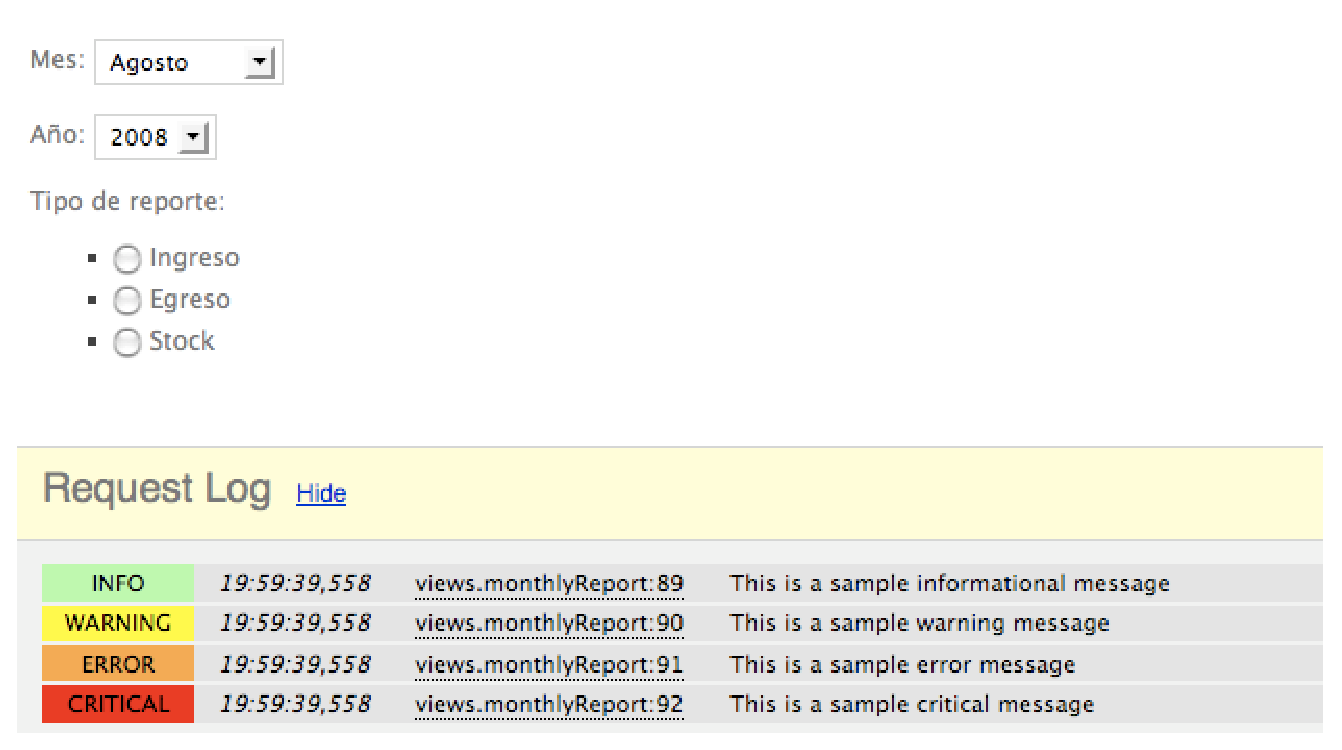
\includegraphics[scale=0.5]{images/django-logging.eps}
	\caption{Resultado de depuración con django-logging}
\end{figure}
 


		\subsection{Depuración basada en puntos de quiebre}
			\subsubsection{Motivación}

Un punto de quiebre es una detención intencional o pausa en un lugar del programa o script, puesto en ese lugar con propósitos de depuración.  En general, un punto de quiebre es el significado de adquirir conocimiento acerca de un programa durante su ejecución.  Durante la interrupción, el programador inspecciona el ambiente de prueba (memoria, archivos, reportes, etc) para averiguar si el programa funciona bien.

			\subsubsection{Proceso de depuración}

En la práctica, un punto de quiebre consiste en una o más condiciones que determinan cuando la ejecución de un programa debe ser interrumpida.  La forma más común de un punto de quiebre es uno, donde la ejecución del programa es interrumpido antes de ejecutar la instrucción especificada por el programador, esto es comúnmente llamado instrucción de punto de quiebre.

Otro tipo de condiciones pueden ser utilizadas, tales como lectura, escritura o modificación de un ubicación específica en el área de memoria.  Esto es comúnmente llamado información de punto de quiebre o un punto de observación.

Los puntos de quiebres además pueden ser utilizados para interrumpir la ejecución en un momento determinado, o cuando se presiona determinada tecla, etc.

Muchos procesadores incluyen soporte de hardware para los puntos de quiebre (comúnmente para los puntos de quiebre de instrucción e información).  Dicho hardware puede incluir limitantes, por ejemplo no permitir puntos de quiebres o instrucciones ubicadas en sectores reservados por el mismo.  Este tipo de restricciones es impuesta por la micro arquitectura del procesador, variando de procesador en procesador.

Sin soporte de hardware, los depuradores tienen que implementar los puntos de quiebre mediante software, lo cual, particularmente para los puntos de quiebre de información, pueden tener un impacto enorme en el rendimiento de la aplicación que esta siendo depurada.


			\subsubsection{Ventajas/Desventajas}

El depurador al momento de encontrar el punto de quiebre, no tiene en sus registros la pila de llamadas que se produjeron, perdiendo toda la información anterior al punto de quiebre.

FALTAN LAS VENTAJAS

			\subsubsection{Herramientas}

				\paragraph{Depurador de Eclipse}
				\paragraph{Depurador Winpdb }	

		\subsection{Depuración Omnisciente}
			\subsubsection{Motivación}

Mediante el registro de cada cambio de un programa en ejecución, es posible presentar al programador cualquier información que desee.  Esencialmente, esto hace posible depurar el programa yendo \textit{atrás en el tiempo}, simplificando bastante el proceso de depuración.


Los desarrolladores de los depuradores se han concentrado completamente en responder la siguiente pregunta: \textit{¿Qué información podemos entregar a los programadores mientras el programa se está ejecutando?}.  Aunque esto no es del todo errado, no es la pregunta correcta.  La pregunta que debieran tener que responder es: \textit{¿Qué información ayudaría más al programador?}.

De estudios informales \cite{} se ha revelado que cientos de programadores, aproximadamente el 90\% de ellos, depuran todos sus programas utilizando sólo instrucciones de impresión.


			\paragraph{Depuración omnisciente}

Un depurador omnisciente trabaja mediante la recolección de eventos generados por cada cambio de estado (cada asignación de variable de cualquier tipo) y cada llamada a un método dentro del programa depurado \cite{odb} \cite{tod}.  Después de terminado el programa es mostrado el depurador (interfaz gráfica) permitiendo al programador ver el estado del programa en el tiempo de ejecución que desee.  

El programador puede seleccionar cualquier variable e ir \textit{atrás en el tiempo} y mirar donde ésta fue definida o cual fue su valor. Existen consideraciones especiales para programas que superan los 10 millones de eventos.


			\subsubsection{Proceso de depuración}

Aunque no existe una definición formal de como llevar a cabo el proceso de depuración en esta técnica, se utiliza la definición de Bil Lewis \cite{odb} para explicar al lector el proceso y componentes esenciales que debe tener un depurador omnisciente.

				\paragraph{Mantener el estado}

Se quiere ser capaz de revertir el programa hacia cualquier estado anterior de ejecución.  Esto implica que debemos grabar cada cambio de cada objeto o variable.  Necesitamos grabar cada asignación en cada hilo de ejecución y definir un orden sobre ellos.  La marca de tiempo debe ser el único referente del estado del programa.

				\paragraph{Presentación}

Cada objeto, variable, instrucción de E/S tendrá un valor conocido para cada marca de tiempo.  Cuando \textit{revertimos el depurador} a un tiempo dado, toda la información es actualizada para reflejar los valores para esa marca de tiempo.

Se muestra toda la información de forma adecuada y el programador no debiera nunca preguntarse ¿ésto cambió? o ¿dónde estoy?

				\paragraph{Identificar el estado}

El programador debe ser capaz de mirar un objeto y saber que objeto es y que valores tienen las variables de instancias.  Los objetos de clases son mostrados justo con el nombre de la clase (ej.: Persona), strings y otras primitivas como se esperan (1, True, ¨soy una cadena¨).

				\paragraph{Navegación}

La simple navegación a través de la historia del programa es dotado a través de la selección de línea en un panel o presionando algunos botones.  Los botones deben trabajar de una forma estándar para los diferentes paneles que existan.


			\subsubsection{Ventajas/Desventajas}

Existen varias razones para hacer un esfuerzo y estudiar la depuración omnisciente:

\begin{itemize}
	\item La primera y más famosa, es fácil depurar cuando puedes ir hacia atrás.  La pregunta más común que los programadores se hacen es ¿Quién definió esta variable?.

	\item Elimina los terribles problemas con depuradores de quiebre, con los cuales el programador debe ¨adivinar¨ en donde poner el punto de quiebre.  No existen pasos extras para depurar, no sucede la situación \textit{fui demasiado lejos}.  Se eliminan los problemas no determinísticos.

	\item Entrega al programador una lista única de eventos del programa siendo capaz de ver las huellas de llamadas a los métodos.

	\item Toda la información es serializada y puede ser analizada remotamente.
\end{itemize}

La gran desventaja de esta técnica se relaciona con la gran capacidad de almacenamiento que se necesita para almacenar las huellas de ejecución.  En el mejor de los casos es adecuado utilizar un cluster.

			\subsubsection{Herramientas}

Algunas de las herramientas que existen en el mercada actualmente son:
\begin{itemize}
	\item EXDAMS
	\item ODB
	\item ZSTEP
	\item TOD
\end{itemize}

	\section{Lenguajes de Programación}

Un lenguaje de programación es un lenguaje que puede ser utilizado para hacer funcionar o controlar el comportamiento de una máquina, particularmente una computadora. Consiste en un conjunto de símbolos y reglas (sintácticas y semánticas), que definen su estructura y el significado de sus elementos y expresiones.

Aunque muchas veces se usa lenguaje de programación y lenguaje informático como si fuesen sinónimos, no tiene por qué ser así, ya que los lenguajes informáticos engloban a los lenguajes de programación y a otros más, como, por ejemplo, el HTML (lenguaje para el marcado de páginas Web).

Un lenguaje de programación permite a uno o más programadores especificar de manera precisa: sobre qué datos una computadora debe operar, cómo deben ser estos almacenados, transmitidos y qué acciones deben tomar bajo una variada gama de circunstancias. Todo esto, a través de un lenguaje que intenta estar relativamente próximo al lenguaje humano o natural, tal como sucede con el lenguaje Léxico. Una característica relevante de los lenguajes de programación, es precisamente que más de un programador pueda tener un conjunto común de instrucciones que puedan ser comprendidas entre ellos para realizar la construcción del programa de forma colaborativa.

Los procesadores utilizados en las computadoras son capaces de entender y actuar según lo indican programas escritos en un lenguaje fijo llamado lenguaje de máquina. Todo programa escrito en otro lenguaje puede ser ejecutado de dos maneras:

\begin{itemize}
	\item Mediante un programa que va adaptando las instrucciones conforme son encontradas. A este proceso se lo llama interpretar y a los programas que lo hacen se los conoce como intérpretes.
	\item Traduciendo este programa al programa equivalente escrito en lenguaje de máquina. A ese proceso se lo llama compilar.
\end{itemize}

		\subsection{Clasificación de los lenguajes de programación}

Los lenguajes de programación se determinan según el nivel de abstracción, según la forma de ejecución y según el paradigma de programación que poseen cada uno de ellos, estos pueden ser:

			\subsubsection{Según su nivel de abstracción}

				\paragraph{Lenguajes de bajo nivel}

Los lenguajes de bajo nivel son lenguajes de programación que se acercan al funcionamiento de una computadora. El lenguaje de más bajo nivel es, por excelencia, el código máquina. A éste le sigue el lenguaje ensamblador, ya que al programar en ensamblador se trabajan con los registros de memoria de la computadora de forma directa.

				\paragraph{Lenguajes de nivel medio}

Existen lenguajes de programación que son considerados por algunos expertos como lenguajes de medio nivel (como es el caso del lenguaje C), al tener ciertas características que los acercan a los lenguajes de bajo nivel pero teniendo, al mismo tiempo, ciertas cualidades que lo hacen un lenguaje más cercano al humano y, por tanto, de alto nivel.

				\paragraph{Lenguajes de alto nivel}

Los lenguajes de alto nivel son normalmente fáciles de aprender porque están formados por elementos de lenguajes naturales, como el inglés. En \textit{BASIC}, el lenguaje de alto nivel más conocido, los comandos como \textit{IF contador = 10 THEN STOP} pueden utilizarse para pedir a la computadora que pare si \textit{contador} es igual a 10. Por desgracia para muchas personas esta forma de trabajar es un poco frustrante, dado que a pesar de que las computadoras parecen comprender un lenguaje natural, lo hacen en realidad de una forma rígida y sistemática.


			\subsubsection{Según la forma de ejecución}

				\paragraph{Lenguajes compilados}

Naturalmente, un programa que se escribe en un lenguaje de alto nivel también tiene que traducirse a un código que pueda utilizar la máquina. Los programas traductores que pueden realizar esta operación se llaman compiladores. Éstos, como los programas ensambladores avanzados, pueden generar muchas líneas de código de máquina por cada proposición o instrucción del programa fuente. Se requiere un proceso de compilación antes de procesar los datos de un problema.

Los compiladores son aquellos programas computacionales, cuya función es traducir un programa escrito en un determinado lenguaje a un idioma que la computadora entienda (lenguaje máquina con código binario).

Al usar un lenguaje compilado, el programa desarrollado no se ejecuta mientras existan errores sintácticos, sino hasta que luego de haber compilado el programa, ya no aparecen estos errores en el código

				\paragraph{Lenguajes interpretados}

Se puede también utilizar una alternativa diferente de los compiladores para traducir lenguajes de alto nivel. En vez de traducir el programa fuente y grabar en forma permanente el código objeto que se produce durante el proceso de compilación para utilizarlo en un proceso de producción futura, el programador sólo carga el programa fuente en la computadora junto con los datos que se van a procesar. Un programa intérprete, almacenado en el sistema operativo del disco, o incluido de manera permanente dentro de la máquina, convierte cada proposición o instrucción del programa fuente en lenguaje de máquina conforme vaya siendo necesario durante el proceso de los datos. No se graba el código objeto para utilizarlo posteriormente.

La siguiente vez que se utilice una instrucción, se debe interpretar otra vez y traducir a lenguaje máquina. Por ejemplo, durante el procesamiento repetitivo de los pasos de un ciclo, cada instrucción del ciclo tendrá que volver a ser interpretado cada vez que se ejecute el ciclo, lo cual hace que el programa sea más lento en tiempo de ejecución (porque se va revisando el código en tiempo de ejecución), pero más rápido en tiempo de diseño (porque no se tiene que estar compilando a cada momento el código completo). 

El intérprete elimina la necesidad de realizar un proceso de compilación después de cada modificación del programa cuando se quiere agregar funciones o corregir errores; pero es obvio que un programa objeto compilado con antelación deberá ejecutarse con mucha mayor rapidez que uno que se debe interpretar a cada paso durante una corrida de producción.

			\subsubsection{Según el paradigma de programación}

Un paradigma de programación representa un enfoque particular o filosofía para la construcción del software. No es mejor uno que otro, sino que cada uno tiene ventajas y desventajas. Dependiendo de la situación un paradigma resulta más apropiado que otro. Atendiendo al paradigma de programación, se pueden clasificar los lenguajes en:


					\paragraph{Paradigma imperativo}
				
Describe la programación como una secuencia de instrucciones o comandos que cambian el estado de un programa. El código máquina en general está basado en el paradigma imperativo. Su contrario es el paradigma declarativo. En este paradigma se incluye el paradigma procedimental (procedural) entre otros.
				
					\paragraph{Paradigma Declarativo}

No se basa en el cómo se hace algo (cómo se logra un objetivo paso a paso), sino que describe (declara) cómo es algo. En otras palabras, se enfoca en describir las propiedades de la solución buscada, dejando indeterminado el algoritmo (conjunto de instrucciones) usado para encontrar esa solución. Es más complicado de implementar que el paradigma imperativo, tiene desventajas en la eficiencia, pero ventajas en la solución de determinados problemas.

					\paragraph{Paradigma Estructurado}

la programación se divide en bloques (procedimientos y funciones) que pueden o no comunicarse entre sí. Además la programación se controla con secuencia, selección e iteración. Permite reutilizar código programado y otorga una mejor compresión de la programación. Es contrario al paradigma inestructurado, de poco uso, que no tiene ninguna estructura, es simplemente un “bloque”, como por ejemplo, los archivos batch o lotes.
				
					\paragraph{Paradigma funcional}
				 
Este paradigma concibe a la computación como la evaluación de funciones matemáticas y evita declarar y cambiar datos. En otras palabras, hace hincapié en la aplicación de las funciones y composición entre ellas, más que en los cambios de estados y la ejecución secuencial de comandos. Permite resolver ciertos problemas de forma elegante y los lenguajes puramente funcionales evitan los efectos secundarios comunes en otro tipo de programaciones.
	
					\paragraph{El paradigma lógico}
				
Se basa en la definición de reglas lógicas para luego, a través de un motor de inferencias lógicas, responder preguntas planteadas al sistema y así resolver los problemas. Ej.: prolog.

	
					\paragraph{Paradigma orientado a objetos}
				
La programación orientada a objetos expresa un programa como un conjunto de estos objetos, que colaboran entre ellos para realizar tareas. Esto permite hacer los programas y módulos más fáciles de escribir, mantener y reutilizar.


Si bien puede seleccionarse la forma pura de estos paradigmas al momento de programar, en la práctica es habitual que se mezclen, dando lugar a la programación multiparadigma.

Actualmente el paradigma de programación más usado debido a múltiples ventajas respecto a sus anteriores, es la programación orientada a objetos.

A continuación se detallan algunas características del lenguaje de programación utilizado en el presente trabajo de memoria para realizar la etapa de implementación.

		\subsection{Python}

			\subsubsection{¿Qué es Python?}

Python es un lenguaje de programación de alto nivel creado por Guido van Rossum a principios de los años 90.  Es un lenguaje similar a Perl, pero con una sintaxis muy limpia y que favorece un código legible.

Se trata de un lenguaje interpretado o de script, con tipado dinámico, fuertemente tipado, multiplataforma y multiparadigma (orientación a objetos, estructurada y funcional).

			\subsubsection{Lenguaje interpretado}

Es un lenguaje de programación interpretado o de script, esto quiere decir que se ejecuta utilizando un programa intermedio llamado intérprete, en lugar de compilar el código a lenguaje máquina que pueda comprender y ejecutar directamente una computadora.

La ventaja de los lenguajes compilados es que su ejecución es más rápida. Sin embargo los lenguajes interpretados son más flexibles y portables.

Python tiene, no obstante, muchas de las características de los lenguajes compilados, por lo que se podría decir que es semi interpretado. En Python, como en Java y muchos otros lenguajes, el código fuente se traduce, la primera que se ejecuta a un pseudo código máquina intermedio llamado bytecode la primera vez que se ejecuta, generando archivos .pyc o .pyo (bytecode optimizado), que son los que se ejecutarán en sucesivas ocasiones.


			\subsubsection{Tipado dinámico}

La característica de tipado dinámico se refiere a que no es necesario declarar el tipo de dato que va a contener una determinada variable, sino que su tipo se determinará en tiempo de ejecución según el tipo del valor al que se asigne, y el tipo de esta variable puede cambiar si se le asigna un valor de otro tipo.


			\subsubsection{Fuertemente tipado}

No se permite tratar a una variable como si fuera de un tipo distinto al que tiene, es necesario convertir de forma explícita dicha variable al nuevo tipo previamente. Por ejemplo, si se tiene una variable que contiene un texto (variable de tipo cadena o string) no se podrá tratarla como un número (sumar la cadena ¨9¨ y el número 8). En otros lenguajes el tipo de la variable cambiaría para adaptarse al comportamiento esperado, aunque esto es más propenso a errores.

		\subsection{Python v/s Java}

Java es un lenguaje cuyos tipos se fijan en el momento de compilar. La mayoría de los lenguajes de tipado estático fuerzan esto exigiéndole al programador que declare todas las varibles con sus tipos antes de usarlas. 

Existen muchas más diferencias entre estos dos lenguajes pero para el caso de estudio sólo nos interesa mostrar esta diferencia como la principal.

INCLUIR TABLA COMPARATIVA.

\chapter{Implementación de depuradores omniscientes}

A lo largo de la historia de la Ciencia de la Computación han existido muchos esfuerzos por implementar depuradores omniscientes, es por esto que se encuentra importante conocer las distintas perspectivas de diferentes equipos de implementación.  A continuación se muestra, dividida por etapas, las distintas implementaciones existentes al día de hoy.

	\section{Implementaciones históricas}

En esta sección se consideran dos implementaciones importantes:
\begin{itemize}
	\item EXDAMS - Extendable Debugging And Monitoring System
	\item ZSTEP - para prolog al parecer
\end{itemize}

		\subsection{EXDAMS}
			\subsubsection{Historia}

Con la llegada de los lenguajes algebraicos de alto nivel, la industria de la computación esperaba ser aliviada de los detalles de programación requeridos en el nivel de los lenguajes ensamblador.  Esta expectativa ha sido en gran parte cumplida y muchos sistemas son ahora construídos en lenguajes de alto nivel.

Sin embargo, la habilidad de depurar programas tiene avances que son pequeños en relación al incremento en el uso de estos lenguajes de alto nivel.  Como Evans and Darlay \cite{} indican:
\textit{¨Nosotros encontramos que, hablando en términos generales, un análisis cercano de casi todas las principales técnicas de depuración de los lenguajes en ensamblador, existe al menos un sistema de depuración perteneciente a algún lenguaje de alto nivel.  Sin embargo, las facilidades de la depuración en linea para los lenguajes de alto nivel son en general menos bien desarrolladas y menos ampliamente usadas (relativo al uso de estos lenguajes) que sus contrapartes para lenguajes en ensamblador¨}.

En general, los sistemas construidos son meramente copias de los depuradores en línea de los lenguajes en ensamblador, más que diseños de facilidades totalmente nuevas para los lenguajes de alto nivel.  Ellos no han creado ni formatos gráficos en los cuales se presente información acerca de la depuración, no han entregado una manera rasonable con la cual los usuarios puedan especificar el proceso requerido en cualquier depurador de información disponible.

EXDAMS, es un intento por quebrar este impase entregando un ambiente simple en el cual los usuarios pueden facilmente añadir nuevas funcionalidades a un depurador en línea sin tener que modificar mayormete el compilador a nivel de código fuente, ni EXDAMS, o sus programas para que sean depurados.


			\subsubsection{Motivación}

EXDAMS, es un sistema depurador y monitor en línea diseñado para facilitar la experimentación con nuevas herramientas de ayuda que cumplan estas mismas características, y para proveer alternancia de forma flexible entre estas ayudas, como el tiempo de ejecución es controlado en cualquiera de los sentidos adelante o atrás.

			\subsubsection{Características}

Es un poderozo depurador y monitor a nivel de código fuente para lenguajes de programación.  Sus facilidades son de dos tipos: estático, el cual hace referencia a un punto específico en tiempo de ejecución; y movimiento, el cual cambia en tiempo de ejecución y puede ser visto, en tiempo de ejecución, sin importar la dirección atrás o adelante (ej.: un usuario puede ver la ejecución de su programa, en reversa, yendo hacía atrás a algún estado anterior).

Adicionalmente, de estas facilidades, las características de ambiente de EXDAMS son:
\begin{enumerate}
	\item Habilidad para alternar, en cualquier punto de ejecución, entre el espacio de los datos (\textit{¿qué está sucediendo?}) y el espacio de control (\textit{¿cómo sucedió esto?}), de esta forma asociando una acción del programa con la instrucción exacta que produce la acción.

	\item Fácil extensión para nuevas herramientas de depuración y monitoreo definidas por el usuario.
\end{enumerate} 

			\subsubsection{Objetivos de diseño}

EXDAMS, fue diseñado para satisfacer tres necesidades:
\begin{itemize}
	\item Como un vehículo para probar algunos propuestas, pero sin aplicarlas, para facilidades de depuración y monitoreo en línea.

	\item Como facilidades extendibles las cuales los nuevos depuradores y monitores pueden añadir fácilmente y luego probarlas.

	\item Como un sistema que provee algunas medidas de independencia de no sólo una máquina en particular sobre la cual está siendo ejecutado este, y la particular implementación de un lenguaje está siendo depurado y/o monitoreado, sino que además de muchos lenguajes fuentes en los cuales los programas de los usuarios pueden ser escritos y depurados, y/o monitoreados.
\end{itemize}

En una situación perfecta para hacer depuración, de acuerdo con la filosofía de EXDAMS, el usuario primero establece \textit{que es lo que está sucediendo}, luego decide si ese comportamiento es correcto, y finalmente, si este no es correcto, determina \textit{como} el programa efectuó esa operación, al mismo tiempo que busca el error en el programa o en la información.  De esta manera, cualquier sistema de depuración y monitoreo exhaustivo debe incluir facilidades poderosas en los espacios de información y control, como también proveer una manera simple de alternancia entre los puntos correspondientes en cualquier espacio, como las necesidades del usuario o preferencias personales le indiquen.

			\subsubsection[Depuración y monitoreo]{Depuración y monitoreo dentro de EXDAMS}

EXDAMS contiene dos tipos de asistencia para la depuración y monitoreo:

\begin{description}
	\item[Asistencia estática] Muestra información que es invariante en relación el tiempo de ejecución (una marca de tiempo es incrementada como cada instrucción del código es ejecutado y usado para referir un punto particular en la ejecución del programa), como son los valores de variables al momento de ocurrir un error, una lista de todos los valores de las variables que fueron dadas en tiempo de ejecución, o una muestra de una porción del código fuente.

	\item[Asistencia dinámica] Esta asistencia es sensible al tiempo de ejecución, esto es, la información que ella muestra puede variar con el tiempo de ejecución.  Esta asistencia dinámica incluye el último valor de \textit{n} de un conjunto de variables, la instrucción actual y la subrutina, además del valor actual del conjunto de variables.  El usuario puede ejecutar la asistencia dinámica en cualquiera de las direcciones, adelante y atrás, controlando el tiempo de ejecución.

\end{description}

Las características más importantes, desde el punto de vista del usuario son:

\begin{itemize}
	\item La habilidad para controlar el tiempo de ejecución de su programa, moviendo una variable rápidamente hacia atrás o adelante, mientras el depurador y/o monitor actualiza constantemente su despliegue de información.

	\item La habilidad de detenerse en cualquier punto en tiempo de ejecución del programa, cambiando al otro asistente, y examinando concienzudamente el comportamiento de su programa.

\end{itemize}

			\paragraph[Análisis de flujo]{Análisis de flujo invertido}

Mediante la llamada de \textit{FLOWBACK FOR}(instrucción reservada de EXDAMS) y especificando un valor en particular, el usuario solicitará a EXDAMS analizar ¿Cómo la información fluyó a través de su programa para producir el valor especificado?.  Este análisis es presentado en la forma de un árbol invertido, con el nodo de más abajo correspondiente al valor del cual el análisis inverso fue solicitado.  Cada nodo consiste en una instrucción de asignación a nivel de código de lenguaje que produjo el valor, el valor mismo, y conectado con los nodos del siguiente nivel.  Estos nodos corresponden a valores no constantes dentro de la instrucción de asignación mostrada que está conectada con esos nodos.  Esos nodos tienen la misma forma como el original y están conectados para todos los valores no constantes utilizados en una instrucción de asignación en particular produciendo su valor.  De esta manera, la siguiente figura muestra en análisis de flujo invertido para un valor particular de A. 

Esta figura muestra que la instrucción de asignación A=B+C-10; produjo un valor específico de A, y este valor fue 105.  Los valores de B y C usado en la asignación de A fue 8 y 107, respectivamente, y fueron producidas mediante las instrucciones de asignación ¨B=R-1;¨ y ¨C=A+E;¨ respectivamente.  Cada uno de los otros nodos se explican de la misma manera.

			\subsubsection{Arquitectura}

EXDAMS es un sistema que cuenta de cuatro fases.  Estas fases son análisis del programa, compilación, recolección de historia y depuración en tiempo de ejecución, con navegación a través de la historia del programa.

				\paragraph{Análisis del programa}

La primera fase analiza el programa fuente del usuario como efectúa las cuatro funciones, la más importante de las cuales es la creación de un modelo para este programa.  Este modelo, el corazón de la fase depuración en tiempo de ejecución con navegación a través de la historia del programa, es la manera por la cual los valores recolectados sobre la cinta de la historia son interpretados y por la cual porciones del código fuente son recuperados, y es el repositorio de toda la información estructural conocida acerca del programa.

En general, la historia contiene toda la información dinámica necesaria para actualizar en tiempo de ejecución cuando se vaya en las direcciones de atrás o adelante, mientras el modelo contiene todo lo necesario sobre la información estática.

El modelo contiene la información estática de control y la información variable de alteración del programa del usuario.  La información de control consiste en la estructura del programa acerca de CALL, GOTO, IF-THEN-ELSE y DO-END, mientras que la información variable de alteración consiste en los nombres de las variables sobre el lado izquierdo los cuales son afectadas por instrucciones de asignación y las cuales a la vez pueden ser alteradas por instrucciones de entrada.

Las instrucciones de depuración añadidas al programa pasan la información relevante de tiempo de ejecución hacia  la recolección de historia en tiempo de ejecución.

				\paragraph{Compilación}

El procesador estándar del lenguaje fuente compila el programa fuente, como actualizado durante el análisis del programa.

				\paragraph[Recolección de historia]{Recolección de historia en tiempo de ejecución}

La versión compilada del programa actualizado es ejecutada con un conjunto de rutinas en tiempo de ejecución que este llama.  Estas rutinas reúnen la información dinámica acerca del comportamiento del programa.

Esta información es completada en un buffer que es escrito cuando se llena.  Esta es la cinta de historia del comportamiento del programa y, junto con la tabla simbolica y el modelo, es suficiente para recrear el comportamiento del programa en cualquiera de las direcciones (atrás o adelante) en el tiempo de ejecución.

				\paragraph[Historia del programa]{Depuración en tiempo de ejecución con navegación a través de la historia del programa.}

Esta fase contiene a los asistentes para depuración y monitoreo los cuales presentan la información histórica hacia el usuario de una manera usable en su pantalla.  Esto además interpreta los comandos del usuario para mostrar alternativas y/o variaciones en tiempo de ejecución, y entrega la capacidad de editar para modificar bug descubiertos y para retornar el programa modificado a las cuatras fases para un nuevo proceso de depuración.


	\section{Implementaciones recientes}

En esta sección consideraremos dos implementaciones importantes:
\begin{itemize}
	\item ODB - Omniscient Debugging
\end{itemize}

		\subsection{ODB}

ODB es una implementación Java la cual recolecta información mediante la instrumentación del byte code del programa objetivo, al momento que éste es cargado.  Este utiliza un mecanismo simple de alto nivel para ordenar los eventos de diferentes hilos.  Este ha sido probado en MacOS, UNIX, y Windows sobre una gran variedad de programas.

Para un depurador gráfico como este, existen dos temas de vital importancia:
\begin{enumerate}
	\item Presentación de la información; ¿Cómo el programador puede obtener desde el depurador, el estado del programa que le interese?
	\item Navegación; ¿Cómo el programador reconoce el estado?
\end{enumerate} 

			\subsubsection{La naturaleza de los bug bajo ODB}

ODB divide a los bug en dos dimensiones:  ¿Todos los eventos registrados para el bug caben en memoria? y ¿El bug produce una información errónea o este falla al producir una información correcta?

				\paragraph{La serpiente en el pasto}

Si el programa imprime \textit{la respuesta 41} en vez de \textit{42}, entonces se tiene un manejador sobre el bug.  Se observa la serpiente en el pasto y se puede agarrar su cola.  Ahora si el programa falla al producir la respuesta correcta, entonces no se tiene un manejador directo del bug, esta es la serpiente en el pasto que no podemos ver.

Para programas en los cuales todos sus eventos son registrados en memoria y en los cuales se pueda ver la serpiente en el pasto, entonces ODB es absolutamente maravilloso.  Es posible comenzar sobre la salida errónea e ir hacia atrás, encontrando el valor inapropiado en cada punto, y luego seguir a este valor hasta su causa. (Si se tiene la cola de una serpiente y se tira lo suficientemente fuerte, se obtendrá su cabeza.)  No es inusual iniciar el depurador, seleccionando la salida errónea, y navegar por el código fuente en 60 segundos, con absoluta confianza.

Los depuradores basados en punto de quiebre sufren del problema \textit{La lagartija en el pasto}.  Incluso cuando ellos pueden ver la lagartija y tirar de su cola, la lagartija quebrará su cola y se irá.  Luego ellos vuelven a otro problema \textit{La lagartija perdida en el pasto}.

Con ODB, existe una versión de este problema.  Cuando la producción incorrecta es causada por la falla de un determinado objeto cuando esta siendo asignado, entonces se tiene que responder la pregunta \textit{¿Quién pudo haber echo esto?}, la cual es una pregunta mucho más difícil que \textit{¿Quién hizo esto?} (Esta es la lagartija sin pata en el problema del pasto).  Nosotros pensamos que tenemos una serpiente, pero después de tirar su cola por un momento, esta la quiebra de cualquier forma.

Para problemas relativamente pequeños (digamos 10.000 eventos), esto es fácil y basta con sólo examinar por completo las huellas de asignación de los métodos.  Para problemas más grandes, la \textit{serpiente perdida en el pasto}, se tornan más problemáticos.  Se tiene una gran cantidad de información acerca de la asignación y una idea no muy cierta de lo que estamos buscando.

Afortunadamente, el problema anterior es un caso profundamente analizado, ODB incorpora la función \textit{get()} de Ducassé (poner referencia!)

				\paragraph{Tamaño}

Otra importante dimensión es la del tamaño.  Dentro de un espacio de direccionamiento de 31-bit, existe espacio para almacenar alrededor de 10 millones de eventos.  Un gran porcentaje de los bug reales encajan dentro de este espacio.  Un buen porcentaje no.  Existe un número de opciones para atacar este problema.  Nosotros podemos:
\begin{itemize}
	\item Recolector de basura, tirar a la basura a los eventos antiguos
	\item Instrumentar pocos métodos
	\item Registrar por poco tiempo 
\end{itemize}

					\subparagraph{Recolección de basura}

Esto es bueno porque no requiere esfuerzo y efectivamente mantiene una ventana de eventos circundante al bug.  Esto de lo contrario es malo porque no se elimina basura, si no que solo eventos antiguos que pudieran ser importantes.  Esto además es malo porque permite el programa correr lo bastante para que el rendimiento se convierta en un tema importante.  Este añade un 50\% extra sobre el mayor de los costos promedio para un evento.

Cuando la fuente del bug está dentro de los 10 millones de evento del tiempo cuando la grabación fue apagada, luego nosotros volvemos el bien conocido problema de "la serpiente en el pasto". Cuando este va más lejos, nosotros perdemos la fuente del bug, y el recolector de basura pierde su valor.

					\subparagraph{Código seguro}

Es muy normal para un gran porcentaje de un programa consista en bien conocido, seguro código fuente. (Existen cualquier metodo recomputable, o metodos que nosotros no queremos ver el interior de ellos).  Mediante solicitud que estos metodos no sea instrumentados, muchos de eventos no interesantes son eliminados.  ODB permite al programar seleccionar arbitrariamente un conjunto de métodos, clases, o paquetes, los cuales pueden ser instrumentados o no.

					\subparagraph{Comenzar detener registro}

Si el programador sospecha que determinado evento conocido siempre ocurre antes del bug (ej.: Cuando presiono este botón el programa se cae), luego el registro puede ser habilitado en ese punto y apagado después del bug.  ODB permite control manual (Existe un botón inicio/fin registro).  Este además permite control automático.  Control automático de la manera que nosotros iremos a examinar un gran conjunto de eventos por un patrón particular, el cual será prendido / apagado registro.  Una vez más, esto es precisamente el problema de los analizadores de eventos para lo cual ODB utiliza la función \textit{get()} de Ducassé.

				\paragraph{Implementación}

ODB mantiene un array sencillo de marca de tiempos.  Cada marca de tiempo es un entero de 32 bit, conteniendo un índice de hilo (8 bits), un indice de linea (20 bits) y un indice de tipo (4 bits).  Un evento para cambiar una instancia de una varible necesita tres palabras: una marca de tiempo, la variable que ha cambiado, y el nuevo valor.  Un evento para una llamada de método necesita: objeto, nombre del método, los argumentos y el valor de retorno (o Excepción), junto con una pequeño montón de variables internas propias del depurador.  Esto añade cerca de 20 palabras.  La instrucción return line además generará 10 palabras más.

Cada variable tiene un historial asociado que es sólo una lista de pares marca de tiempo / valor. Cuando el ODB quiere saber cual valor de una variable fue en el tiempo 102, este justo agarra el valor que está más cerca al valor previo.  La lista de historia para variables locales y argumentos cuelgan sobre la Linea de huella.

Siempre que ocurra un evento, este bloquea por completo el debugger, una nueva marca de tiempo es generada y registrada dentro de la lista, y estructuras asociadas son construidas.  Los valres de retorno y excepciones son agregadas dentro de la apropieda linea de huella como ellas fueran generadas.

La inseción en el código es muy simple.  El byte code fuente es examinado y un código instrumentado es insertado antes de cada asignación y cerca de cada llamada de método.

Una inserción tipica luce de esta forma:

\begin{verbatim}
289 aload 4											// nuevo valor
291 astore_1										// variable local ie
292 ldc_w #404 <String ¨Micro4:Micro4.java:64¨>
295 ldc_w #416 <String ¨ie¨>
298 aload_1											// ie
299 aload_2											// Huella padre
300 invokestatic #14 <change(String, String, Object, Trace)>
\end{verbatim}

Donde el código original eran las lineas 289 y 291, asignando un valor a la variable local \textit{ie}.  La instrumentación crea un evento que registra que sobre la linea 64 de Micro.java(\#292), la variable local ie(\#295), de quien su Lista de historia puede ser encontrada sobre la linea de huella en el registro 2 (\#299), le fue asignada al valor en el registro 1 (\#298).  Los otros tipos de eventos son similares.


	\section{TOD: depurador omnisciente para Java}
		\subsection{Contribución}

La contribución de este trabajo es mostrar que la depuración omnisciente puede ser realizada a través del uso de diferentes técnicas mejorando factores como la eficiencia, escalabilidad y usabilidad.  Lo planteado es validado por TOD, un depurador portable orientado a la huella para Java integrado dentro de ECLIPSE [5].  Las características de TOD son:
\begin{description}
	\item[Eficiente generación de eventos] Basado en un compacto modelo de huella, un uso de codificación binaria de eventos, y un rápido tejedor de bajo nivel.

	\item[Máquina especializada de base de datos distribuida] Para un almacenamiento escalable y rápido y consultas sobre eventos, que aprovecha la muy limitada naturaleza de la ejecución huellas.  En unos 10 nodos dedicados en cluster TOD mantiene una tasa sustancial de entrada de 170.000 eventos por segundo y cientos de consultas por segundo.

	\item[Soporte para huellas parciales] Ofreciendo mecanismos estáticos y dinámicos para la generación selectiva de la huella y un reporte adecuado para la información incompleta.

	\item[GUI informativa] Debido a la eficiencia del procesamiento de consultas TOD es utilizado para depurar una aplicación compleja como eclipse preservando su interactividad.

	\item[Componentes especializados de GUI] Entregando una vista de alto nivel en huellas grandes de eventos para una navegación mucho más efectiva, como el mural de hilos.
\end{description}


		\subsection[Desafíos]{Desafíos del debugging omnisciente}

	Se presentan las características principales de un degugger omnisciente comparado con los debuggers tradicionales y el perfil de los desafíos de escalabilidad del debugging omnisciente.

			\subsubsection[Características]{Características de un debugger omnisciente}

	Un debugger omnisciente(OD; DO) entrega cuatro características principales:
\begin{itemize}
	\item Paso (stepping)
	\item Estado de reconstitución
	\item Reconstitución del control del flujo
	\item Encontrar la causa principal.  
\end{itemize}
El último es una característica única de los debuggers omnisciente, mientras que las otros son características de los debuggers típicos.

	En debuggers basado en punto de quiebre, stepping consiste en la ejecución del programa objetivo una instrucción a la vez.  Existen dos variaciones del stepping:  step over ejecuta el método sin estar esperando dentro del llamado del mismo, mientras el step into espera a la primera instrucción (comienzo) de la llamada del método.  Reconstitución del estado consiste en ir entregando al programador un objeto de estado inspector cuando el programa objetivo está esperando.  Reconstitución del control de flujo permite obtener una vista en la llamada de la pila actual del programa, con ligadura a variables y objetos.  OD's extiende estas tres características con completa libertad en relación al tiempo:  stepping puede ser realizado tanto hacia adelante como hacia atrás, los programadores pueden inspeccionar el estado de objetos como estaban en cualquier punto del tiempo, y pueden libremente navegar por el árbol de control.

	Finalmente, una de las características más usadas de OD's es su habilidad para encontrar \textit{dónde} y \textit{en qué contexto} a un campo o variable en particular le fue entregado un determinado valor.  Frecuentemente los bugs se manifiestan mucho después de suceder su causa principal.  Para ejemplo, tratar de referirnos a una referencia NULL obtenida desde un campo dado causa una caída, esto es el síntoma del bug.  La información que el programador necesita saber es dónde el campo fue definido con el valor NULL.  Con un debugger basado en punto de quiebre, incluso si la ejecución es pausada justo antes del imperfecto referido, la causa raíz del bug pudo haberse perdido.  Ejemplo:  porque el código que causó el problema ya no está más en la pila de llamadas.

			\subsubsection{Desafío de escalabilidad}

Destacando las características presentadas sobre la necesidad de generar y registrar las huellas de ejecución.  El potencial crecimiento de estas huellas plantean diversos desafíos de escalabilidad, cuando son la principal razón que afecta a la calidad de producción de OD's.

Los eventos deben ser grabados rápidamente, preferentemente en tiempo real, como que  (a) debugging puede comenzar inmediatamente después que el programa objetivo haya terminado o caído, y (b) el desbordamiento en tiempo de ejecución es minimizado para preservar sobre todo el desempeño del programa depurado y la interactividad cuando se necesite (ejemplo debugging Eclipse).

El debugger puede causar una interferencia mínima al programa objetivo en el sentido de no afectar su comportamiento.  En particular, la administración del espacio de direcciones y de memoria del proceso objetivo no puede ser alterado.

La capacidad del almacén de eventos de un debugger omnisciente debe estar alineado con un número esperado de eventos dentro del uso total de la huella; con GHZ CPU's, cientos de millones de eventos pueden ser generados en solamente pocos minutos de ejecución.


Fig. 1 Arquitectura de alto nivel de TOD

Consultas dentro la huella de ejecución deben ejecutarse a una velocidad compatible con la interacción del usuario; por ejemplo: en décimas de segundos para operaciones como el stepping.
La información debe ser presentada de una manera que trata que la carga cognoscitiva de la navegación a través de la enorme huella de los eventos sea la menor posible, permitiendo una rápida identificación de los bug's.

 	Este trabajo se encamina en el uso optimizado de las representaciones de los eventos e indexación agresiva, un modelo simple de consulta, soporte para una una base distribuida, soporte para huellas parciales y componentes de presentación e interacción especializados.

		\subsection{Acerca de TOD}

TOD es un debugger orientado a la huella para Java, que se dirige sobre la identificación del uso de la escalabilidad.  El objetivo es dirigir esos usos en el orden para obtener un debugger omnisciente que es prácticamente aplicable.  Esta sección da un panorama de TOD en el sentido de su arquitectura, el modelo de evento, y los componentes de la GUI.

			\subsubsection{Arquitectura}

TOD es diseñado basándose en dos ideas centrales:

\begin{itemize}
	\item Desacoplar el núcleo del debugger desde el programa objetivo en ejecución.
	\item Ser portable.  
\end{itemize}

Esto es hecho sobre un árbol de componentes (Fig.1):  el objetivo (JVM) en el cual el programa depurado se ejecuta y emite eventos, el núcleo del debugger que implementa las principales funcionalidades de TOD, y la interfaz del debugger a través del cual el usuario a la misma vez consulta y navega en la huella de ejecución.

La racionalidad para almacenar los eventos en una base de datos preferentemente que están en memoria como huellas en otros debuggers omniscientes [8,13,15] está precisamente dirigido a algunos de los desafíos discutidos en la sección 2.2.:  almacenando eventos en el espacio de dirección del  objetivo de la aplicación no es escalable para unos cuantos cientos de megabytes de información de la huella, e interfiere con el administrador de memoria, en particular con el colector de basura.  El costo de captura se incrementa por el uso de una base de datos que es compensado por una mejor escalabilidad y sin generar intrusión.  Como efecto secundario esto permite a los depuradores post-morten tener la habilidad de serializar la huella de ejecución, lo que abre una interesante perspectiva para las compañías de software dispuesta a ofrecer software con alta calidad de soporte:  observando el costo de almacenamiento, una huella de ejecución navegable es una información lejos mucha más relevante para reportar un bug que un texto descriptivo apropiado. 

Tabla 1.  Eventos y sus atributos

La cabecera de las filas son tipos de eventos y la cabecera de las columnas son posible argumentos (ts: tiempo, tid: identificador del hilo, depth: llamada a la pila en profundidad, pev: puntero al padre del evento, LOC: localidad del código fuente, fid: identificador de celda, bid: identificador del método, vid: identificador de variable local, idx: índice, val: valor, ret: valor de retorno, tgt: objetivo, vxc: excepción; args: argumentos).

Durante la ejecución, la aplicación objetivo emite eventos que son enviados al núcleo del debugger, donde ellos son grabados e indexados en una base de datos de eventos.  El tema de los eventos que son emitidos es discutido posteriormente.  La base de datos de los eventos contiene las particularidades del curso del evento y el conjunto restrictivo de posibles consultas que entrega entre el alto rendimiento de grabación y el buen desempeño de las consultas (ver en sección 4 y 5).  El núcleo del debugger contiene otra base de datos, la base de datos estructural, que contiene información estática sobre la aplicación objetivo.  En particular realiza un seguimiento de identificadores de 32 bits que son asignados a elementos estructurales del programa objetivo(por ejemplo: clases, métodos y campos(celdas)).  Las consultas son efectuadas por el usuario basándose entre el evento y la base de datos estructural.

			\subsubsection{Representación y emisión eventos}

Introducimos ahora a la representación de los eventos y las huellas de estos, así como también los eventos son emitidos por la aplicación depurada en TOD.

\begin{description}

	\item[Modelo de evento y huella] Un evento es una estructura caracterizada por un número de atributos elegidos entre el conjunto A={a0,...,ak}.   Observemos e.aj el valor del atributo aj del evento e.  Para cada j perteneciente [0...k], dejamos Dj como el dominio de aj, por ejemplo el conjunto de todos los valores distintos que pueden ser tomados por aj, para cualquier evento dentro de la huella.  Una huella del evento T=$<$e1,...,en$>$ es una secuencia ordenada de n eventos heterogéneos.

El atributo a0 corresponde al timestamp del evento; este es caracterizado por el hecho que (a) todos los eventos tienen un valor para a0, (b) allí existe un completo orden sobre D0 y (c) los eventos en T están ordenados por sus valores de a0.  Tabla 1 muestra cuales eventos concretamente son capturados y cuáles son sus atributos.

	\item[Emisión de los eventos]  El núcleo del debugger de TOD captura los eventos emitidos por la aplicación objetivo (Fig. 1).  Existen tres vías en las cuales los eventos pueden ser emitidos:  puertos especializados de la huella del hardware [7],  maquina virtual o interpretador de instrumentación [14], y aplicación de instrumentación [8, 13]].  TOD utiliza la última:  aunque no es tan rápida como las pruebas de hardware y significativamente utiliza más espacio que el nivel de instrumentación de máquina virtual en términos de tamaño de código, la instrumentación de aplicación es mucho más portable y fácil de implementar.

En TOD, la JVM que está alojada en la aplicación objetivo está configurada para usar el agente  JVMTI\footnotemark[1] .  El agente intercepta los eventos cargados por la clase y reemplaza las definiciones originales por la versión instrumentada.  Instrumentación es realizada por el tejedor en el núcleo del debugger:  el agente envía el bytecode original al núcleo,  el tejedor implementa la clase y almacena estructuradamente la información en la base de datos estructural, y la clase modificada es enviada nuevamente a la JVM objetivo donde es eventualmente cargada (Fig. 1).  El agente toma la clase instrumentada del disco duro para reducir el número de turnos de los procesos internos.  Esto es  particularmente usado por el uso frecuente de las clases como algunas en el JDK.

\footnotetext[1]{Interfaz de herramienta de la máquina virtual de Java, parte de la plataforma de Java 5.}

La instrumentación se efectúa utilizando la librería de bytecode ASM [3]:  el código de captura  del evento es añadida antes y/o después de un patrón especifico de bytecode en el código original, tal como un campo de escritura o una llamada a un método.  Cuando el código instrumentado es ejecutado, los eventos son construidos a partir de sus atributos, serializados en un formato binario personalizado, y enviados través de un socket a la base de datos de eventos.

	\item[Sincronización no ambigua del evento] Aunque los timestamps del evento son obtenidos a través del servicio de precisión en nano segundo de Java, es potencialmente carente de exactitud haciendo posible que varios eventos del mismo hilo tengan el mismo valor timestamps.  Como esto es incompatible con el esquema de indexación usado por TOD, se cambió el valor original del timestamp por unos bits a la izquierda y se usan los bits libres para diferenciar eventos del mismo hilo que sea parte del mismo timestamp.  Cuando se compara el timestamps de los eventos de diferentes hilos, se usa el timestamp original para preservar el orden de los hilos internos(inter-thread).

	\item[Alcance de la captura de huella] El esquema de instrumentación descrito anteriormente es selectivo, esto es, es posible de proveer filtros definidos para los usuarios que limite el número de eventos emitidos.

	\item[Identificación del objeto] El agente JVMTI de TOD asigna un único identificador para cada objeto en la aplicación objetivo.  Como una excepción a este mecanismo las instancias de los objetos que representan valores primitivos (por ejemplo entero, decimal, etc) tales como las cadenas y exceptions son pasadas por valor.
\end{description}

			\subsubsection[Bajo nivel de consultas]{Bajo nivel de consultas: cursores y contadores}

	Todas las características presentadas en la sección 2.1 (paso a paso, reconstitución de estado, reconstitución del control de flujo y encontrar la causa raíz) pueden ser expresados en términos de dos niveles de consultas de bajo nivel:  cursores y contadores, que introducimos a continuación.  Ambos basados en el filtrado de eventos de la huella de acuerdo a algunas condiciones de sus atributos.  Condiciones que pueden ser cualquier combinación booleana de simples predicados de la forma attribute = value, donde value es una constante.  Para la instancia (kind = FW o kind = BC) o target = obj145.  Si Q es una condición y e es un evento, definimos el predicado de la función Q(e) cuyo valor es verdadero si e verifica la condición Q.

	La actual posición del cursor está representado por la linea negra entre los eventos cuatro y cinco.  Los Eventos que juntan el predicado del cursor están en gris.   llamamos sucesivamente a next() retornando los eventos 5,6,11 y 14;  llamando posNext(11) la posición del cursor entre los eventos 10 y 11; llamando posPrev(11) las posiciones estarán entre los eventos 11 y 12.

Fig. 2 Navegación entre la unión de los eventos y el predicado del cursor 
operación
semántica {significado}
next() / prev()
Retorna el siguiente / previo unión de eventos y mueve el cursor hacia adelante / atrás.
posNext(t) / posPrev(t)
Mueve de modo que la siguiente llamada a next()/prev() retorna el primero/ultimo evento cuyo timestamp es mejor / peor que o igual que t.
posNext(ev) / posPrev(ev)
Mueve de modo que la siguiente llamada a next() / prev() retorne el evento dado.
Tabla 2. operaciones de los cursores

\begin{description}
	\item[cursores] Definimos cursor(Q) como un iterador sobre los eventos que reúnen la condición Q (Fig. 2).  Los cursores tienen una posición actual que está situada entre dos eventos consecutivos (o hacia el principio o el término de la huella).  Un cursor soporta un número de operaciones de navegación, como las mostradas en la tabla 2.

	\item[contadores] Entregan un intervalo de tiempo [t1,t2] dividido en s porciones de largo delta t = (t1 ‚Äì t2)/s cada uno, y una condición Q para los atributos del evento, una consulta de contador regresa un arreglo de s enteros tales que s[i] = | \{e pertenece a T: dentro(e, t1 + i*delta t) and Q(e)\} | donde dentro(e,t) < = > e.ts > = t  and e.ts < t + delta t.   Cada posición del arreglo contiene el número de eventos unidos Q que ocurrieron durante la correspondiente porción de tiempo.
\end{description}

			\subsubsection{Alto nivel de consultas}

A continuación se explica como los cursores y los contadores son combinados algoritmicamente para implementar el alto nivel de las características descritas anteriormente.

\begin{description}
	\item[Stepping] Definimos stepper como un objeto que tiene un evento actual ev y soporta operaciones paso hacia adelante y hacia atrás, paso dentro y paso sobre.  Por ejemplo, paso hacia adelante dentro es definido como sigue:

	c <-- cursor(thread = ev.thread)
	c.posPrev(ev); ev <-- c.next()


Paso hacia adelante sobre cambia la condición del cursor a: thread = ev.thread and depth = ev.depth.  Paso atrás es simétrico al paso hacía atrás.

	\item[Reconstitución de estado] El valor v de una celda f de un objeto en particular o con tiempo t puede ser recuperado como sigue:

	c <--cursor(kind = FW  and fid = f and target = o)
	c.posPrev(t); v <-- c.prev().val

El estado de un objeto puede ser recuperado realizando la misma operación para cada uno de los campos.  La pila de marcos son reconstituidos en una manera similar, usando eventos de escritura variables instanciados de la celda de eventos escritos.

	\item[Reconstitución del control de flujo] Los eventos que ocurren en el alto nivel del control de flujo de una llamada dada del método e  son recuperados de la siguiente manera:

	c <-- cursor(thread = e.thread  and depth = e.depth + 1)
	c.posPrev(e.ts); cflow = <>
	repeat
		ev = c.next(); cflow <-- cflow union <ev>
	until ev.kind = Bex

	\item[Buscador de la causa inicial] Determinando como a un campo ha sido asignado un valor indeseado es tan directo como la consulta de la reconstrucción del estado:  en lugar de obtener el valor del evento de la celda escrita que asignó el valor al campo, el evento por si mismo se hace el actual, dando acceso para el contexto en ese momento.  La exploración atrás en el tiempo es la causa que pueda ir sobre esto, encima de la causa inicial.
	
\end{description}

			\subsubsection{Componentes de la interfaz gráfica}

La interfaz de TOD puede ser usada independiente o como una añadidura para el IDE de Java llamado Eclipse (Fig. 3).  El navegador de usuario entre diferentes vistas utiliza las ampliamente conocidas metáforas de los navegadores web (hyper vínculos, botón hacia atrás).  Las vistas disponibles son:  inspector de objetos, control de flujo, y mural.  

\begin{description}	
	
	\item[Vista de inspección de objetos] Muestra la reconstitución de objetos, y permite encontrar la causa inicial por valor de celdas a través de un conveniente ¿por qué? link a cada campo siguiente. 
	
	\item[Vista de control de flujo] Muestra una constitución del flujo de control y permite las operaciones de stepping así como encontrar la raíz de la causa para valores de variables locales.


	\item[murals] Las descripciones del nivel alto son útil para marcar patrones anormales del comportamiento.  Sin embargo representando un número fuerte de eventos en un limitado número de píxeles es difícil.  Jerding y Stasko introdujeron la información del mural [9] como una \textit{reducción de la representación de la información del espacio entero a uno que se ajusta enteramente dentro de una ventana mostrada}.  Las características de los eventos murals de TOD, los cuales son gráficas que muestran la evolución de la densidad del evento, o un número de eventos por unidad de tiempo, en un periodo dado.  Por ejemplo, TOD puede mostrar la densidad del evento por cada uno de los hilos para el conjunto de ejecución de la aplicación objetivo (Fig. 4), o la densidad de llamadas a métodos de un objeto en particular.  Las densidades son obtenidas a través  de los contadores, donde el largo de las tajadas de tiempo correspondiente al espacio utilizado por un simple pixel de la barra en el mural.  El usuario puede hacer un acercamiento y ver el murals;  cuando el nivel de acercamiento permite distinguir los eventos individuales del usuario puede seleccionar un evento y ver el contexto dentro.
	
\end{description}

Botón (A) lanza el programa con el trace registrando la huella.  El usuario navega en el control de flujo (B) utilizando los botones de paso (C), o por medio de un click sobre el evento.  La linea correspondiente al evento actual está resaltada en la ventana del código (D).  El estado de la pila de marcos y el objeto actual es mostrado en la ventana (E).  El usuario puede saltar de una instrucción que defina el valor actual de una variable o campo por medio de un click en why? Siguiendo a este.


Fig. 3 Stepping con TOD en Eclipse

de una vista de paso.  El mural de hilos tiene distintas aplicaciones, por ejemplo: entender la interoperación entre los hilos, o spotting dead y las livelocks.

		\subsection{Soporte para base de datos de alta velocidad}

Ahora describimos y analizamos el esquema de indexación de TOD, el cual permite la ejecución eficiente de consultas mientras es lo suficientemente rápida para permitir un alto rendimiento de grabación.

La necesidad para desarrollar una cimiento de base de datos especializada para TOD fue motivado por el bajo rendimiento del uso profundo de la administración de sistemas de base de datos para nuestros propósitos: PostgreSQL y Oracle sólo soportan almacenar eventos a una taza de 50 y 500 eventos por segundo respectivamente, mientras nuestros registros la taza está en el orden de los cientos de millones de eventos por segundo [19].  Nuestro alto rendimiento especializado en los cimientos de la base de datos permiten la siguiente especificaciones para el stream del evento de 

El gráfico muestra la densidad de los eventos a lo largo del eje del tiempo.

una huella de ejecución: (a) el stream del evento es de sólo lectura, (b) los eventos al llegar son ordenados a partir del timestamp y (c) las consultas son limitadas por el filtrado.

			\subsubsection{Indexación jerárquica de los eventos}

TOD adopta un esquema de indexación jerárquica que permite recuperar al evento juntando un predicado en orden según su timestamp sin tener que acceder realmente a los eventos en si, reduciendo así los costos del procesamiento de consultas.

\begin{description}
	\item[Indices en los valores de los atributos] Usando la notación definida anteriormente, se define el índice de T en aj como una función Ij: Dj --> (Do,N)* j pertenece [1..k] de modo que ningún mapa Ij tenga cualquier posible valor v de aj una secuencia de índices de entrada de la forma (ts,i).  Una entrada aparece en el índice Ij(v) si y sólo si ei.aj = v and ei.a0 = ts, donde ei es el i-esimo evento de T.  Adicionalmente, las entradas son ordenadas por ts.  Esos indice pueden ser usados directamente para recuperar todos los eventos que correspondan a una consulta simple de la forma attribute = value.
	
	\item[Jerarquía de indexación por timestamp] Debido a que las consultas en TOD no consisten sólo en encontrar eventos correspondientes que ocurrieron antes o después de un momento, los índices son ordenados por sus valores de ts, entonces es posible presentarlos en una búsqueda binaria para encontrar el timestamp deseado.

Esto es siempre mucho más eficiente para extender el índice de estructura en una manera jerárquica (Fig. 5).  Cada índice jerárquico para el valor v del atributo aj contiene un número de niveles;  El índice Ij(v) describe sobre la constitución del nivel 0.  La entrada (ts, i) índice del nivel 0 son almacenados en el disco duro en pequeñas páginas, donde cada una contiene un número de entradas pertenecientes al mismo índice.  Cuando una página está llena, una entrada de la forma (ts,pid) es creada en el índice del nivel 1: ts es tomado desde la primera entrada (ts,i) de la reciente pagina llena, y pid es un puntero a esa página.  Las entradas del Nivel 1 están acumuladas en una página; cuando una página del Nivel 1 es llenada, una entrada en el Nivel 2 es creada, y así sucesivamente.  

El nivel más alto siempre contiene una pagina sencilla, llamada la página raíz.  El número de niveles sobre el Nivel 0 de un índice es llamado la altura del índice.  
\end{description}


			\subsubsection{Costo de la creación de un índice}

Los experimentos muestran que el tamaño promedio de un evento es ||e||= 50 bytes.  El tamaño de una entrada de Nivel 0 es (ts,i) = 16 bytes (dos enteros de 64 bits).  El tamaño de las entradas de nivel superior es (ts,pid) = 12 bytes (pid está en 32 bits).  Las experiencias han determinado que el tamaño de una página óptima es P = 4096 bytes, por lo tanto los indices de las páginas de Nivel 0 contienen 256 entradas, en los niveles superiores las páginas contienen 341 entradas y las paginas de eventos contienen 81 eventos en promedio.  La altura h de los índices es logarítmica con respecto al número de entradas y en la práctica nunca excedieron 5 (un índice de altura 5 permite para 341 and 5 ~ 4x10 12 entradas)  Asumiendo que la actual página de eventos puede residir en memoria, la página de eventos sólo causa una página escrita cada 81 eventos.

Para cada evento que entre a la base de datos a lo más existirá k = |A|-1 índices que actualizar (como no hay índice separado en a0).  Los experimentos indican que el promedio k = 10.  Dado ciertos eventos que llegan en orden con respecto a a0, actualizando un índice sólo pensando en añadir una entrada en el final de la página en el Nivel 0, y en el final de las paginas de nivel superior sólo cuando un página de nivel inferior es llenada.  La entrada/salida y costos de memoria de esta operación son los siguientes:

\begin{itemize}
	\item Si la página de índices actual para cada nivel puede residir en memoria, un costo de E/S es realizado sólo cuando una pagina está llena.  El número promedio de páginas accedidas por el evento entrante es:

	\item Si sólo la pagina de índices está en el nivel 0 puede ser mantenida en memoria, cuando una página es llenada debe ser escrita, El nivel de la página leída es el 1, actualizado y escrito en el disco.  Analizando, el nivel más alto, tiene aproximadamente 0.13 accesos por evento.  

	\item Si la pagina no puede ser mantenida en memoria, cualquier actualización implicará las tres operaciones anteriores, entregando 20 accesos por evento.
\end{itemize}

	La cantidad de memoria dedicada al buffering de página es por lo tanto lo más importante:  Hay una diferencia de  400 directorios entre la situaciones extremas anteriores.

	Ahora se estima el número total de índices, sumatoria de j=1 hasta k sobre | Dj |, en orden de determinar cuántas páginas de buffer de memoria se necesita para permanecer en el caso donde al menos la página actual del nivel 0 para que cada índice quepa en memoria.  Los atributos de los eventos pueden ser divididos en dos categorías.  El dominio de los atributos estáticos (por ejemplo: behavior id, field id, type id, ubicación, etc.) depende solamente de la estructura del programa, no del tamaño de la huella.  En las pruebas con la captura de las huellas en Eclipse, se observó que estos acumulan cerca de 200.000 distintos valores.  Hay dos atributos dinámicos: thread id y object id.  Su dominio puede ser enorme dado que el programa objetivo puede repetitivamente crear y destruir objetos e hilos durante su ejecución.  Sin embargo, sólo una fracción de ellos puede ser usado en cualquier punto dado en el tiempo:  Todos los objetos que viven deben ajustarse dentro de la JVM's objetivo que está disponible en memoria y todos los hilos que viven deben ser razonablemente ejecutados por la CPU.  Así es solamente necesario tener un espacio para el índice del buffer de la pagina para los objetos e hilos usados actualmente.

	El dominio de los  object id's claramente domina todos los dominios acumulados.  Si la aplicación objetivo regularmente usa un millón de objetos, cerca P*10 \^ 6 = 4GB de espacio es necesario para el buffer, el cual es alcanzable por el actual mid-end systems.


			\subsubsection{Costo de recuperación del evento}

	Ahora se presenta los algoritmos que permiten recuperar eventos buscando un predicado arbitrario en la linea de tiempo con respecto al tamaño de los índices involucrados.  Los algoritmos son recuperados en orden respecto a su timestamp; la recuperación al revés tiene el mismo costo.

\begin{description}
	\item[condiciones simples] Para una condición simple de la forma aj = C donde C es una constante, podemos recuperar eventos buscados ordenados por timestamp, simplemente obteniendo las entradas (ts,i) desde Ij(C).  Si el evento actual es requerido (por ejemplo: por los cursores), estos son directamente recuperados desde la huella como ei; si no (por ejemplo: para los contadores) el evento no necesita ser accedido.  En cualquier caso, todas las entradas pueden ser recuperadas en la linea de tiempo, debido a que el índice se explora simplemente una vez.

	\item[condiciones conjuntivas] Para una conjunción booleana de una condición simple de la forma aj1 = C1 \^ .... \^ ajm = Cm, nosotros usamos una variante del algoritmo sort merge join[2], extensamente utilizado en la administración de los sistemas de bases de datos, para identificar los eventos buscados sin accesarlos (Algoritmo 1):  obtenemos el Ij1 (Cl) para cada una de las condiciones simples, y por cada uno mantenemos un puntero a la entrada actual (tsl,il).  Entonces iteramos: en cada paso verificamos si todos los il son iguales, en este caso añadimos cualquier resultado a las entradas actuales:  El echo que todos ellos hacen referencia al mismo evento significa que el evento coincide con todas las condiciones.  Entonces avanzamos el puntero de índice cuya entrada actual tenga el mínimo valor para ts.  Como cada índice es revisado una sola vez y no existen ciclos anidados, merge join corre en tiempo lineal con respecto a la suma de los tamaños de los índices considerados.
\end{description}

		\subsection{Medidas de rendimiento}

Se presentan reportes sobre el primer conjunto de medidas de rendimientos evaluando diferentes aspectos de TOD:

\begin{itemize}
	\item Base de datos distribuida, en terminos de registro de eventos y evaluación de consultas.
	\item Sobrecarga que efectuada por la emisión de eventos en la aplicación depurada.
\end{itemize}

			\subsubsection{Desempeño de la base de datos}


Para evaluar el rendimiento de la base de datos distribuida de TOD, se han realizado varias mediciones de rendimientos en relación al registro y consultas bajo distintas configuraciones.  Se capturó una gran huella de ejecución de una sesión de Eclipse donde el usuario realizó un simple secuencia de pasos: Abrió un archivo escrito en Java, lo editó utilizando completación automática, creando una nueva clase y la editó. La huella capturada comprende aproximadamente 516 millones de eventos y pesa 20GB.  Luego se importó esta huella dentro de la base de datos de TOD, que utiliza 16 nodos dedicados dentro de un cluster.  En este experimento hasta 10 nodos estaban para ser utilizados como nodos de base de datos, y 1 como disparador y agregador de consultas.  Cada nodo es un Intel Itanium de 1.60GHZ con 2GB de RAM y 7GB espacio disponible en el disco duro local, corriendo un kernel Linux 2.6.9 y BEA JRockit 1.5.0 06 JVM.  Los nodos están conectados a través de un adaptador de red de 1Gbps.  Desafortunadamente esta no es una configuración ideal para TOD.

La primera medida de rendimiento es el tiempo tomado para importar la huella de ejecución dentro de la base de datos.  La segunda medida de rendimiento es la taza en la cual eventos individuales coinciden con una condición arbitraria pueden ser recuperados utilizando un cursor, y la tercera medida de rendimiento es el tiempo tomado para computar los contadores de eventos de estos mismos para la duración completa de la huella.

\begin{description}
	\item[Registro] Primero se determinó la tasa de transferencia máxima del disparador mediante la desactivación del procesador de eventos en relación a los nodos de la base de datos:  El disparador puede manejar hasta 200.000 eventos por segundo, independientemente del número de nodos (Fig. 7)  Los resultados actuales muestran que una nodo de base de datos es capas de manejar aproximadamente 50.000 eventos/segundo, y que con 10 nodos se obtiene limitar al disparador cerca de los 170.000 eventos/segundo (fig. 8).  El rendimiento incrementa con el uso de más nodos, aunque no muy linealmente.  La comparación es sin embargo basada por el echo que con pocos nodos , menos eventos fueron importados.  Se puede conjeturar que el rendimiento obtenido con pocos nodos habría sido menor si se hubiera sido capas de importar la huella completa.
	
	\item[Cursores de consultas]  Se midió la velocidad de ejecución de dos tipos de cursores de consultas stepping-related:  seek y step.  Ambas están basadas sobre en una condición compuesta generada aleatoriamente que se ajusta con eventos de determinado hilo de ejecución y profundidad de la llamada.  La búsqueda de las peticiones de las consultas de un cursor con una condición, posición que en un timestamp elegidas al azar en el lapso de ejecución de la traza y obtener el siguiente evento que corresponda.  La operación es repetida 1.000 veces, cada tiempo con diferentes condiciones y timestamp.  Las consultas de paso (step) además solicita un cursor similar y se posiciona en un timestamp aleatorio, pero luego trae los siguiente 1.000 eventos correspondientes.  La operación es repetida cien veces.
	
Los resultados se muestran en Tabla 3(a).  En este experimento se utilizaron un tamaño fijo de eventos de huellas de 80 millones de eventos la cual puede ser importado en una base de datos usando 3 de los 10 nodos.  La eficiencia de consultas de búsqueda no mejora, e incluso decrece, cuando más nodos de base de datos son utilizados.  Este es porque cada consulta de búsqueda recupera solo un evento, el cual obviamente está presente en un solo nodo.  El tiempo de buscar ese evento es por lo tanto igual al máximo del tiempo tomado por cada nodo para encontrar el siguiente evento que corresponda, entregando la condición de la consulta y el timestamp. Las consultas de paso son un poco más rápidas cuando más nodos son utilizados pero sorprendentemente la mejora está lejos de ser lineal.  Aún no se ha encontrado todavía una explicación para este resultado inesperado.  A pesar de una débil capacidad de ampliación (Fig. 9), la posición del cursor de consultas se ejecuta en décimas de segundos, lo suficientemente rápido para ser utilizado interactivamente a través de la interfaz de depuración de TOD.		
	\item[Contadores de consultas]  Se midió la velocidad de ejecución de los contadores de consultas y se compararon dos métdos: merge counts y fast counts.  Se utilizó una porción de la huella de ejecución de Eclipse descrita anteriormente, que contenía 80 millones de eventos distribuidos en 27 hilos de ejecución.  Se solicitaron al contador de eventos por cada hilo sobre el lapso de la huella, dividiendo n = 1.000 subintervalos.  Los resultados son entregados en Tabla 3(b) y la escalabilidad es representada en la Fig.9.  Varios puntos que son importantes de destacar:

		\begin{itemize}
			\item Contadores rápidos proveen una aproximación bastante precisa, con una distorsión por bajo del 2\% de comparación con los resultados reunidos de los contadores. La distorsión fue calculada: 

			\item Contadores rápidos son mucho más rápido que los contadores de fusión, pero no mejoran en relación al aumento de nodos en la base de datos, debido a que cada nodo registra menos eventos, el algoritmo de contador rápido debe recurrir frecuentemente a indices de niveles inferiores.
 
			\item Los contadores de fusión escalan linealmente, en términos de números de nodos.
		\end{itemize}
\end{description}

			\subsubsection{Sobrecarga por emisión de eventos}

En el sentido de evaluar la sobrecarga de la emisión de los eventos, se compara el tiempo de ejecución de un programa (a) independiente, (b) con TOD y (c) con ODB, otro depurado omnisciente para Java.  Como en esta medida de rendimiento se desea medir la sobrecarga por emisión de eventos cuasado por TOD y no el rendimiento de su base de datos, los eventos simplemente son escritos en el disco sin indexación.

El programa objetivo es un programa de prueba que hace uso intensivo de CPU, el cual crea 100 instancias de objetos y luego itera 10 millones de veces en un cilco que toma uno de estos objetos de forma aleatoria y le pasa un metodo que efectúa una simple operación aritmética sobre su código hash.  El programa no llama a ningún método no instrumentado y por esto que cada operación emite un evento.
 
Esta prueba de rendimiento fue realizada en un Pentium M de 2GHz notebook con 1GB de ram corriendo el kernel 2.6.17 de Linux y la JVM 1.5.0 08 de Sun.  Los resultados son presentados en la Tabla 4.  Como los eventos en ODB son almacenados en la pila de la JVM del programa objetivo; los eventos antiguos son eliminados cuando la pila está llena.  Se realizaron dos pruebas con ODB, cambiando el tamaño de la pila de la JVM.  Con 500MB de la pila se fue capas de registrar 5 millones de eventos de 110 millones emitidos durante la ejecución del programa.  Con 64MB se pudo registrar solo 500.000 eventos.  Por otra parte con TOD se fue capa de registrar 90 millones de eventos emitidos sin interferir con la pila de la JVM.  La huella de ejecución generada pesa 3.6GB.  La sobrecarga de la emisión de eventos es similiar en TOD y en ODB: alrededor de 115 veces la de TOD, donde los eventos son serializados y escritos en disco.

Se debe hacer notar que esta medida de rendimiento representa el peor escenario.  Se midió la sobrecargar de uso intensivo de CPU, instrumentando completamente un programa, mientras que en las situaciones típicas de depuración algunas partes de los programas son excluidos de la instrumentación, como se expondrá posteriormente

			\subsubsection{Discusión}

Los resultados experimentales presentados anteriormente muestra que es factible registrar y consultar grandes huellas de ejecución para el propósito de la depuración omnisciente.  Se fue capas de registrar una huella de ejecución de 20GB correspondiente a una sesión de trabajo en Eclipse, un IDE bastante complejo orientado a Java, y se importó sobre los 400 millones de eventos de esa huella en la base de datos distribuidas para eventos a una tasa de 170.000 eventos/segndo, cercano a tres veces más lento que la tasa máxima de eventos observada, 520.000 eventos/segundo.  La base de datos fue también capas de servir entre 5 y 350 cursores de consultas por segundo y producir contadores globales de consultas para 27 hilos de ejecución en menos de 10 segundos; cada tiempo de respuesta es compatible con los requerimientos de interactividad de la interfaz de usuario del depurador.  Se utilizó la base de datos distribuida sobre un cluster dedicado y realizando medidas utilizando 1 hasta 10 nodos de la base de datos.  La base de datos demostró escalabilidad por cada evento registrado y consultas, pero no tanto para los cursores de las consultas. Por lo que respecta a la emisión de eventos la sobrecarga es preocupante, se observó que un intensivo uso de CPU, de un programa completamente instrumentado ejecutado bajo TOD disminuye alrededor de 115 veces y emite alrededor de 520.000 de eventos/segundo.  Este caso es similar al obtenido con ODB, un depurador omnisciente que almacena eventos en un espacio de direcciones en el proceso objetivo y de esta forma no es tan escalable.  En esta implementación el disparador de eventos impone un embotellamiento de 200.000 eventos/segundo; Una mejor implementación del disparador (presumiblemente en C) es necesario si las huellas de ejecución son grabadas en tiempo real.




		\subsection{Trabajando con huellas parciales}

	Aunque TOD está diseñado para soportar grandes huellas de ejecución, no siempre es practicable grabar cada evento:  El tiempo de ejecución mayor de una captura de evento es importante, como también lo es los requerimientos de almacenamiento.  La idea de las huellas parciales es que se puede afirmar el echo que durante el desarrollo de una pieza de software, algunos componentes son confiables, por ejemplo: maduros y bien probados, y por esto no es necesario generar y almacenar eventos para las actividades internas de esos componentes.  Esta sección muestra como el alcance de la captura de la huella puede facilitar el debugging y como TOD hace posible el trabajo con huellas parciales.

			\subsubsection[Ejemplo de motivación]{Ejemplo de motivación: Depurando el plugin de TOD en eclipse}

Consideremos como un ejemplo de depuración el mismo plugin de TOD en eclipse.  Este ejemplo es bastante representativo de un componente de desarrollo existente, probado, frameworks o arquitecturas de plugin.  Aquí, se está fuertemente interesado en dos tipos de bugs:  aquellos que son internos del plugin y aquellos que relacionados con la interacción entre el plugin y la plataforma.  En el primer caso, nosotros no necesitamos capturar eventos que ocurren dentro de la plataforma ECLIPSE porque eso es considerado como probado.  En el segundo caso, nosotros tenemos que grabar eventos que ocurren dentro de la plataforma, pero no necesariamente todos:  puede que sean bastantes los eventos que se deban grabar de la Java Tooling(JDT), o solamente alguna parte de ella, por ejemplo la interfaz de usuario.

Figura 10 muestra el impacto de diferentes alcances de estrategias de la huella en comparación con el número de eventos emitidos y el exceso del tiempo de ejecución, durante diferentes etapas de la ejecución del plugin de TOD.  En este pequeño experimento podemos ver que por apropiado que sea el alcance de la captura de la huella, hay sobre cinco ordenes de magnitud de diferencia en el número de eventos emitidos, y que los aumentos en el exceso del tiempo de ejecución puede ser sobre 20 tiempos, realza enormemente la aplicabilidad de TOD.

			\subsubsection{Tratando con información incompleta}

El inconveniente de ignorar algunos eventos es que la captura de la huella de ejecución es incompleta, y por lo tanto, alguna información es precaria para reconstruir la historia completa del programa.  El soporte para huellas parciales de ejecución en TOD es conseguida mediante reportes sistemáticos, sobre la información perdida, al usuario para que el pueda razonar sólidamente acerca de la información disponible.  La información pérdida se manifiesta en dos áreas: cuando el código no instrumentado es llamado desde un código instrumentado, y en el turno de las llamadas de código instrumentado, alguna información sobre el flujo de control es perdida; en este caso TOD entrega indicadores visuales en los lugares apropiados, como se muestra en la figura 11.  Segundo, en el estado de reconstitución: si una clase tiene un atributo no privado que es escrito por código no instrumentado, el valor de este campo en un punto determinado del tiempo no puede ser determinado de forma exacta.  TOD representa estos campos con un color distinto en las correspondientes vistas.


Los pequeños puntos indican que la información del flujo de control pudo ser perdida: El método Collections.sort no está instrumentado pero llama al método de comparación de la clase instrumentada Comp durante su ejecución

         Fig. 11. Reportando una información de flujo de control potencialmente incompleta.


\chapter{pyTOD}
	\section{Arquitectura de pyTOD}
		\subsection{Modelo de componentes}

Para tener una mejor perspectiva de los componentes que componen pyTOD, es que se utiliza el diagrama de componentes del lenguaje unificado de modelamiento UML.  Es importante señalar que este diagrama en ningún caso es un diagrama de bajo nivel.		
\begin{figure}[hpb]
	\centering
	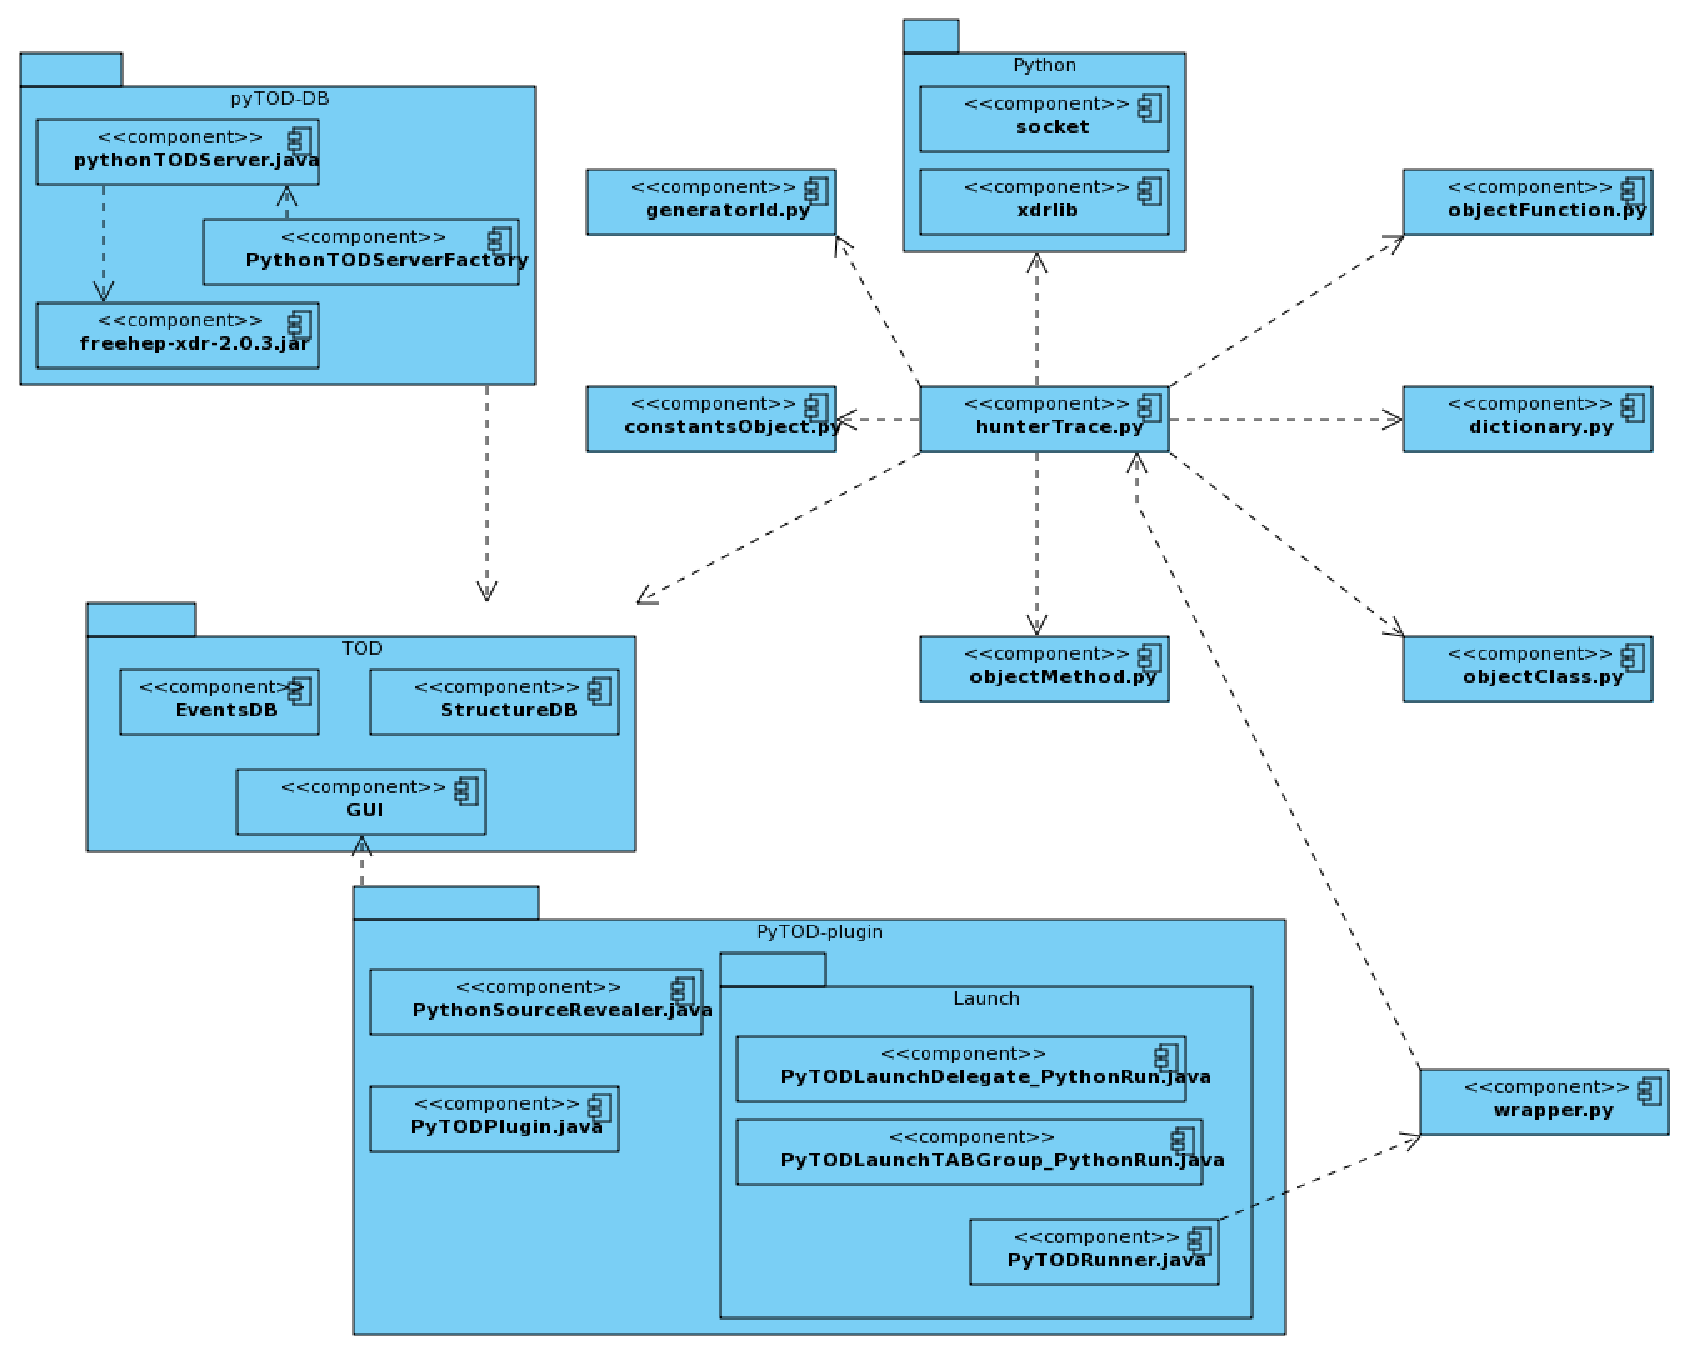
\includegraphics[scale=0.5]{images/componentModelHunterTrace.eps}
	\caption{Diagrama de componente del capturador de huella}
\end{figure}	
		
		
		\subsection{Wrapper}
		
Por un asunto de usabilidad se ha construido un wrapper con el objetivo que el programador no deba modificar ninguna linea de los script que desee depurar.  A continuación su muestran dos ejemplos, el primero sin utilizar el wrapper y el segundo utilizando el wrapper.

\begin{itemize}
	\item Código sin wrapper
\begin{singlespace}
\begin{lstlisting}[style=Python]
import sys
sys.path.append('/Volumes/archivos/eclipse/workspace/python-project/src')
from debugger.pytod.core.hunterTrace import hT

class miClase(object):
    def __init__(self, y):
        self.condicion = True
        self.cantidad = 1
        self.metodo(self.z, 1, 2, 3)
        return
    
    def metodo(self, h, i, j, k):
        self.cantidad = 1 + h
\end{lstlisting}
\end{singlespace}

Como se puede observar el programador añadió tres lineas (lineas desde la uno hasta la tres) a su código, tema que se vuelve tedioso al momento de modificar cientos de archivos en los cuales está distribuido su software.  Para evitar esto es que se construyó el wrapper, el cual evita que el programador tenga que introducir lineas de código ajenas a su programa.  

	\item Código con wrapper

A continuación se muestra el código fuente del wrapper:
	
\begin{singlespace}
\begin{lstlisting}[style=Python]
import sys
from debugger.pytod.core.hunterTrace import hT

print "PyTOD wrapper v1"
if __name__ == '__main__':
    #print sys.argv
    execfile('\%s'\%(sys.argv[1]),locals(),globals())
\end{lstlisting}
\end{singlespace}

Básicamente wrapper implementa las lineas que en el caso anterior el programador tuvo que agregar a su script, además wrapper de lo anterior wrapper se encarga de ejecutar el script del programador.  Wrapper es utilizado en el plugin construido para Eclipse.

\begin{singlespace}
\begin{lstlisting}[style=Python]
class miClase(object):
    def __init__(self, y):
        self.condicion = True
        self.cantidad = 1
        self.metodo(self.z, 1, 2, 3)
        return
    
    def metodo(self, h, i, j, k):
        self.cantidad = 1 + h       
\end{lstlisting}
\end{singlespace}
\end{itemize}

Como se puede observar el programador, en este caso, no tiene la necesidad de modificar su programa.

\begin{figure}[hpb]
	\centering
	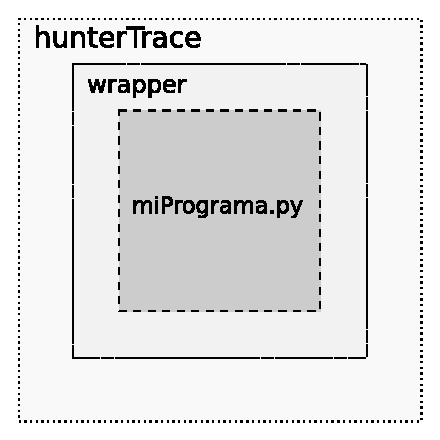
\includegraphics[scale=1]{images/wrapper.eps}
	\caption{Diagrama de composición wrapper}
\end{figure}
		
		\subsection{Diagrama general}
	
	
	\section{El Modelo y Diseño de pyTOD}
	
	Diagrama de comunicación, diagrama de clases
	
\begin{figure}[hpb]
	\centering
	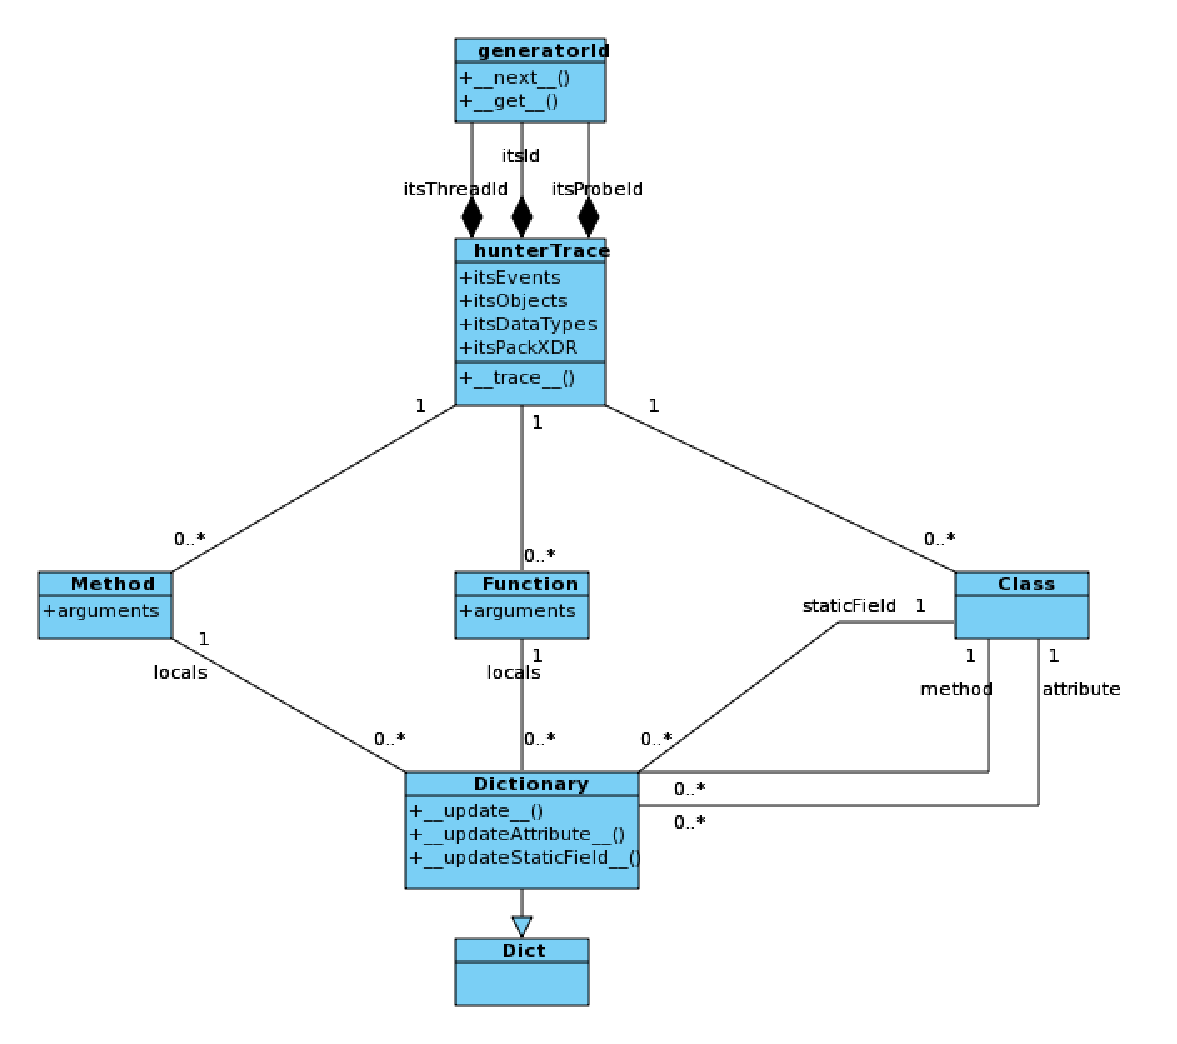
\includegraphics[scale=0.6]{images/classModelHunterTrace.eps}
	\caption{Diagrama de clase del capturador de huella}
\end{figure}
	
	
	\section{Implementación de pyTOD}
		\subsection{Capturador de huella}
		
El capturador de huella es el encargado de: a) registrar la estructura del programa objetivo (clases, métodos, funciones, atributos de instancia, atributos de clase, variables locales, threads, probes) y b) capturar los eventos que este genere en tiempo de ejecución (Llamadas a métodos/funciones, asignaciones/modificaciones, instanciaciones, retornos de métodos/funciones, excepciones). 

El capturador de huella tiene una dependencia directa con la función \textit{settrace} \cite{settrace} perteneciente al módulo estándar \textit{sys}.  Esta función por definición fue creada para facilitar la creación de depuradores de código.

Es por lo anterior que en el presente trabajo de memoria se utilizó esta función para satisfacer ciertos requerimientos de registro estructural del programa objetivo.  Es importante señalar que la función settrace no cubre todas las necesidades de este trabajo de memoria, ejemplo: no es posible estar enterado de la creación o modificación de una variable de instancia o una variable de clase.

A continuación se muestra un ejemplo a nivel introductorio como esta función trabaja:

\begin{itemize}
	\item{Programación estructurada}

\begin{singlespace}
\begin{lstlisting}[style=Python]
import sys

def trace(aFrame, aEvent, aArg):
    if aEvent == 'call':
        print "Llamada a", aFrame.f_code.co_name
        return trace
    elif aEvent == 'line':
        print "Ejecutando linea", aFrame.f_lineno, 
        return trace
    elif aEvent == 'return':
        print "Saliendo de", aFrame.f_code.co_name, 
        print "con valor", aArg
    elif aEvent == 'exception':
        pass

sys.settrace(trace)

def miFuncion(aPrimero, aSegundo):
    if aPrimero > aSegundo:
        theResultado = aPrimero + aSegundo
    else:
        theResultado = aPrimero - aSegundo
    return theResultado

if __name__ == '__main__':
    theResultado = miFuncion(10,5)
    print "Mi resultado es:", theResultado
\end{lstlisting}
\end{singlespace}

El resultado que obtenemos al ejecutar este código es:
\begin{singlespace}
\begin{lstlisting}[style=consola, numbers=none]
peregrino:~ minostro$ python miTrace.py
Llamada a miFuncion
Ejecutando linea 20
Ejecutando linea 21
Ejecutando linea 24
Saliendo de miFuncion con valor 15
Mi resultado es: 15
\end{lstlisting}

	\item{Programación Orientada a Objetos}
\begin{lstlisting}[style=Python]
import sys

def trace(aFrame, aEvent, aArg):
    if aEvent == 'call':
        print "Llamada a", aFrame.f_code.co_name
        return trace
    elif aEvent == 'line':
        print "Ejecutando linea", aFrame.f_lineno, 
        print "indice bytecode", aFrame.f_lasti
        return trace
    elif aEvent == 'return':
        print "Saliendo de", aFrame.f_code.co_name, 
        print "con valor", aArg
    elif aEvent == 'exception':
        pass

sys.settrace(trace)

class miClase(object):

    def __init__(self):
        pass
    
    def miMetodo(self, aPrimero, aSegundo):
        if aPrimero > aSegundo:
            theResultado = aPrimero + aSegundo
        else:
            theResultado = aPrimero - aSegundo
        return theResultado

if __name__ == '__main__':
    theClase = miClase()
    theResultado = theClase.miMetodo(5, 10)
    print "Mi resultado es:", theResultado
\end{lstlisting}
\end{singlespace}

El resultado que obtenemos al ejecutar este código es:
\begin{singlespace}
\begin{lstlisting}[style=consola, numbers=none]
peregrino:~ minostro$ python miTrace.py
Llamada a miClase
Ejecutando linea 18
Ejecutando linea 20
Ejecutando linea 23
Saliendo de miClase con valor {'miMetodo': <function miMetodo at 0x82eb0>, '__module__': '__main__', '__init__': <function __init__ at 0x82e70>}
Llamada a __init__
Ejecutando linea 21
Saliendo de __init__ con valor None
Llamada a miMetodo
Ejecutando linea 24
Ejecutando linea 27
Ejecutando linea 28
Saliendo de miMetodo con valor -5
Mi resultado es: -5
\end{lstlisting}
\end{singlespace}
\end{itemize}

Es importante dejar en claro la diferencia entre los sucesos estructurales y los eventos.  A continuación se detalla cada uno de éstos, se explica su implementación y ejecución dentro del capturador de huella:

			\subsubsection{Sucesos estructurales}
			
				\paragraph{Registro de clase}

El objeto clase se registra junto a sus métodos en el momento que el programador termina de definirla.  El capturado de huella al detectar el evento \textit{return}, preguntará en el diccionario \textit{frame.locals} si es que la función \textit{\_\_init\_\_} está presente como atributo en este diccionario, de ser así, el capturador de huella registrará la definición de la clase.  Ejemplo:

\begin{singlespace}
\begin{lstlisting}[style=Python]
class miClase(object):

    def __init__(self):
        pass
    
    def miMetodo(self, aPrimero, aSegundo):
        if aPrimero > aSegundo:
            theResultado = aPrimero + aSegundo
        else:
            theResultado = aPrimero - aSegundo
        return theResultado
\end{lstlisting}
\end{singlespace}

Es importante señalar que la clase se registra cuando existe un evento \textit{return} debido a que Python al momento de finalizar la construcción de la clase, carga todo el diccionario del \textit{frame} en el atributo \textit{aArg} del evento \textit{return} \cite{bytecode} 

\begin{singlespace}
\begin{lstlisting}[style=consola,numbers=none]
"""
Contenido de aArg
"""
{
	'miMetodo': <function miMetodo at 0x82eb0>, 
	'__module__': '__main__',
	'__init__': <function __init__ at 0x82e70>
}

\end{lstlisting}
\end{singlespace}

Como se puede observar en esta estructura de datos se encuentran todos los métodos de la clase que serán ligadas el objeto en el momento de instanciación.  Luego de registrar la clase en el diccionario de la clase hunterTrace, se envía un mensaje a través de un socket a la base estructural de TOD para crear un registro relacionado con la clase:

\begin{singlespace}
\begin{lstlisting}[style=consola,numbers=none]
Registrando clase miClase
\end{lstlisting}
\end{singlespace}

Continuando con el registro completo de la clase se guardan los métodos definidos en ella.  Los métodos son almacenados en una estructura de datos especial perteneciente a la clase objectClass.

Finalmente, se registran los atributos de clase de la misma forma que se registran los métodos.  Estos atributos son guardados en una estructura de dato especial de la clase objectClass.  Este caso se trata con mayor complejidad que el anterior, debido a que la estructura de la base de datos TOD no permite registrar un atributo de clase que esté fuera de un métido de la clase, situación que en Python se definen como atributos de la clase a cualquier variable que esté dentro del cuerpo de la definición de la clase y fuera del cuerpo de los métodos definidos para esta.  Bajo esta situación se tomó la decisión de crear en el lado Java un método artificial llamado \textit{\textbf{clase}StaticMethod}, al cual se le asociarán todos los atributos de clase que se encuentren en la situación descrita anteriormente.


				\paragraph{Registro de método}

El registro de método se realiza en el momento que se detecta un evento del tipo \textit{call}.  Se busca en el diccionario \textit{locals} del frame la llave \textit{self}, si está en el diccionario, se utiliza para obtener la clase a la cual pertenece el método.  Para obtener la clase asociada al método se realiza lo siguiente:

\begin{singlespace}
\begin{lstlisting}[style=consola,numbers=none]
type(self).__name__
\end{lstlisting}
\end{singlespace}


Con este nombre se busca la clase en \textit{hunterTrace} y se obtiene el identificador único del método para poder registrarlo en la base de datos estructural de TOD:

\begin{singlespace}
\begin{lstlisting}[style=consola,numbers=none]
Registrando el metodo miMetodo id = 105
\end{lstlisting}
\end{singlespace}

Es importante selañar que al momento de registra un método en la base de datos estructural se deben enviar los argumento de esta.  Por definición Python pone como primer argumento la referencia a la instancia, la forma estándar de nombrarlo es self, este argumento no es registrado como argumento en la base de datos estructural.

Los argumentos son registrado utilizando como identificador la posición que ocupan en \textit{frame.f\_code.co\_varnames}, que por definición son siempre los primeros elementos que contiene esta estructura de datos.

				\paragraph{Registro de método especial}

De la misma forma que se registra un método se registra este método especial.  Como anteriormente se señala este método artificial se utiliza al momento de registrar un atributo de clase.  Este método siempre se encontrará por el nombre \textit{\textbf{Clase}SpecialMethod} siendo Clase el nombre de la clase a la cual pertenece.

A este método no se le registran argumentos ni variables locales.  Este método es registrado en la base de datos estructural de TOD la primera vez que se registra un atributo de clase.

\begin{singlespace}
\begin{lstlisting}[style=consola,numbers=none]
Registrando el metodo especial miClaseStaticMethodid = 106
\end{lstlisting}
\end{singlespace}

				
				\paragraph{Registro de función}
				
En el caso de este registro se busca en \textit{locals} el atributo \textit{self}, de no encontrarse se verifica que el objeto sea una función utilizando la función \textit{isfunction} del módulo \textit{inspect}.  De ser una función esta se registra en la base de datos de TOD.			

\begin{singlespace}
\begin{lstlisting}[style=consola,numbers=none]
Registrando la funcion miFuncion id = 115
\end{lstlisting}
\end{singlespace}

Respecto a los atributos la única diferencia es que no se tiene que omitir el atributo self ya que para funciones esto no existe.


				\paragraph{Registro de atributo de instancia\label{registerField}}

La función de sistema \textit{settrace} no entrega ningún mecanismo para estar notificado de la creación de un atributo de instancia.  Es por esto que se utiliza en mecanismo llamado \textit{\_\_setattr\_\_} que es un método interno de Python \cite{setattr} que permite estar notificado en el momento que se asigna un valor o se modifica una variable de instancia.  Lo que se hace es sobrescribir este método para todas las clases que el programador haya escrito.

Se muestra un ejemplo de funcionamiento de este método:

\begin{singlespace}
\begin{lstlisting}[style=Python]
class Descriptor(object):
    def __setattr__(self, aName, aValue):
        """
        Metodo de interes que permite auditar los movimientos
        de las variables de instancia
        """
        if aName in self.__dict__:
            print "Modificacion de", aName, "por el valor", aValue
        else:
            print "Registro de", aName, "con el valor", aValue
        object.__setattr__(self, aName, aValue)

class miClase(Descriptor):
    
    def __init__(self):
        self.itsEdad = 15
        self.itsSexo = "Masculino"
        self.itsColor = ("Amarillo", "Verde", "Azul")
    
    def modificaEdad(self, aEdad):
        self.itsEdad += aEdad

if __name__ == "__main__":
    theClase = miClase()
    theClase.modificaEdad(20)
\end{lstlisting}
\end{singlespace}

El resultado de la ejecución es la siguiente:

\begin{singlespace}
\begin{lstlisting}[style=consola,numbers=none]
peregrino:~ minostro$ python miDescriptor.py
Registro de itsEdad con el valor 15
Registro de itsSexo con el valor Masculino
Registro de itsColor con el valor ('Amarillo', 'Verde', 'Azul')
Modificacion de itsEdad por el valor 35
\end{lstlisting}
\end{singlespace}

Como se puede ver funciona todo de forma correcta, pero se detectó un problema de usabilidad de cara al programador.  Cada vez que el programador defina una clase deberá heredar de Descriptor, cosa que para un par de clases no es molesto pero cuando este número se incrementa puede llegar a ser molesto e incomodo para el programador.

Como solución a lo anterior se agrega directamente al diccionario local en el momento de la definición de la clase el método \textit{\_\_setattr\_\_} de la clase \textit{Descriptor}

\begin{singlespace}
\begin{lstlisting}[style=consola,numbers=none]
theLocals.update(
    {
        '__setattr__':Descriptor.__dict__['__setattr__']
    }
)
\end{lstlisting}
\end{singlespace}

Finalmente el atributo de instancia es registrado en la base de datos.

\begin{singlespace}
\begin{lstlisting}[style=consola,numbers=none]
h0 - fieldWrite   (thread: 101, p.ts: 1217048770743326976, depth: 2, ts: 1217048770744072960, fid: 118 (x), target: UID: 117, val: 6
\end{lstlisting}
\end{singlespace}


				\paragraph{Registro de atributo de clase\label{registerStaticField}}

Para realizar este registro se debe diferenciar dos situaciones importantes:
\begin{enumerate}
	\item Si el atributo de clase se encuentra definido en el cuerpo de la clase pero fuera del cuerpo de los métodos, se utilizará el mecanismo de registro señalado para esta situación en el registro de clase [citar sección].
	\item Si el atributo de clase está definido dentro de un método de la clase, se utilizará el paradigma de metaprogramación.
\end{enumerate}

Se muestra un ejemplo para mostrar su funcionamiento:

\begin{itemize}
	\item Atributo de clase definido dentro del cuerpo de la clase pero fuera del cuerpo de los métodos
	\item Atributo de clase definido dentro del cuerpo de los métodos

\begin{singlespace}
\begin{lstlisting}[style=Python]
class MetaDescriptor(type):

    def __setattr__(self, aName, aValue):
        """
        Metodo de interes que permite auditar los movimientos
        de las variables de clase
        """    
        if aName in self.__dict__:
            print "Modificacion de", aName, "por el valor", aValue
        else:
            print "Registro de", aName, "con el valor", aValue
        super(MetaDescriptor, self).__setattr__(aName, aValue)
        
        
class miClase:
    
    __metaclass__ = MetaDescriptor
    
    def __init__(self):
        self.__class__.itsEdad = 73
        self.__class__.itsColor = "Rojo"
    

if __name__ == "__main__":
    theClase = miClase()
    miClase.theSexo = "Femenino"
    miClase.itsEdad += 1
\end{lstlisting}

El resultado de la ejecución del código es el siguiente:

\begin{lstlisting}[style=consola,numbers=none]
peregrino:~ minostro$ python miMetaDescriptor.py
Registro de itsEdad con el valor 73
Registro de itsColor con el valor Rojo
Registro de theSexo con el valor Femenino
Modificacion de itsEdad por el valor 74
\end{lstlisting}

\end{singlespace}

Al igual que en el caso del registro de atributos de instancia es incomodo para el programador personalizar su clase para que pueda comportarse de la manera que se desea, es por esto que en el momento de definir la clase se agrega al diccionario locals el atributo \_\_metaclass\_\_ con valor MetaDescriptor.

\begin{singlespace}
\begin{lstlisting}[style=consola,numbers=none]
theLocals.update(
    {
        '__metaclass__':MetaDescriptor
    }
)
\end{lstlisting}
\end{singlespace}
\end{itemize}
Es importante que de ambas formas se logra registrar el atributo de clase en la base estructural de TOD.

\begin{singlespace}
\begin{lstlisting}[style=consola,numbers=none]
Registrando un atributo estatico con id 108
\end{lstlisting}
\end{singlespace}


				\paragraph{Registro de variable local\label{registerLocal}}
				
El registro de una variable local puede realizarse en dos situaciones:

\begin{enumerate}
	\item Si el programador escribe explícitamente la instrucción \textit{return} en el método o en la función, todos los registros de las variables locales se realizarán cuando suceda el evento \textit{line}.
	\item Si el programador no escribe explícitamente la instrucción \textit{return}, en el método o en la función, los registros de las variables locales se realizarán cuando sucedan los eventos \textit{line} y \textit{return} \cite{bytecode}.
\end{enumerate}

En ambos casos se asegura el registro de la variable local en la base de datos estructural de TOD.

\begin{singlespace}
\begin{lstlisting}[style=Python]
Registrando variable local: y
\end{lstlisting}
\end{singlespace}

La forma de capturar la creación de una variable local, es inspeccionando el byte code de Python en búsqueda de la instrucción \textit{STORE\_FAST}. \cite{bytecode}

Es importante señalar que al momento de registrar el método o la función se crea un lnotab \cite{lnotab} propio que es una estructura de datos que indica los rangos de los indices del byte code, para luego ser consultados al momento de inspeccionar el byte code.  Esto se realiza para hacer un poco más eficiente el proceso de búsqueda dentro del bytecode.

Se muestra un ejemplo introductorio para graficar la forma en que se registran los variables locales.

\begin{singlespace}
\begin{lstlisting}[style=Python]
import sys
import dis

class miTrace:
    def __init__(self):
        self.itsLnotab = None

    def __createlnotab__(self, aCode):
        theLnotab = {}
        if hasattr(aCode, 'co_lnotab'):
            table = aCode.co_lnotab
            index = 0
            last_index = None
            for i in range(0, len(table), 2):
                index = index + ord(table[i])
                if last_index == None:
                    last_index = index
                else:
                    theLnotab.update({index:tuple([last_index,index-1])})                
                    last_index = index
            theLnotab.update(
             {
               len(aCode.co_code)-1:tuple(
                  [last_index,len(aCode.co_code)-1])
             })                
        return theLnotab 
    
    def __getpartcode__(self, aCode, aLimits):
        theLower = aLimits[0]
        theUpper = aLimits[1]
        theCode = aCode.co_code
        theStoreFast = {}    
        while theLower < theUpper:
            theOp = ord(theCode[theLower])
            theNameOp = dis.opname[theOp]
            theLower = theLower + 1
            if theOp >= dis.HAVE_ARGUMENT:
                theValue = ord(theCode[theLower])
                theValue += ord(theCode[theLower+1])*256
                theLower = theLower + 2
                if theOp in dis.haslocal and \
                theNameOp == 'STORE_FAST':
                    theArgumentValue = aCode.co_varnames[theValue]
                    theStoreFast.update({theArgumentValue:theValue})
        return theStoreFast

    def trace(self, aFrame, aEvent, aArg):
        theCode = aFrame.f_code
        if aEvent == 'call':
            print "Llamada a", aFrame.f_code.co_name
            print "Byte Code asociado:"
            dis.disassemble(theCode)
            print "1. Generando lnotab = ",
            self.itsLnotab = self.__createlnotab__(theCode)
            print self.itsLnotab
            print "2. Comienza inspeccion"
            return self.trace
        elif aEvent == 'line':
            if self.itsLnotab.has_key(aFrame.f_lasti):
                theByteCodeLocals = self.__getpartcode__(theCode,self.itsLnotab[aFrame.f_lasti])
                print "[line] Examinando rango:", self.itsLnotab[aFrame.f_lasti],
                print ", resultado de inspeccion:", theByteCodeLocals
            return self.trace
        elif aEvent == 'return':
            if self.itsLnotab.has_key(aFrame.f_lasti):
                theByteCodeLocals = self.__getpartcode__(theCode,self.itsLnotab[aFrame.f_lasti])
                print "[return] Examinando rango:", self.itsLnotab[aFrame.f_lasti],
                print ", resultado de inspeccion:", theByteCodeLocals        
            print "Saliendo de", aFrame.f_code.co_name, 
            print "con valor", aArg
        elif aEvent == 'exception':
            pass

sys.settrace(miTrace().trace)
\end{lstlisting}
\end{singlespace}

Código donde el programador escribe la instrucción \textit{return}:

\begin{singlespace}
\begin{lstlisting}[style=Python]
def miFuncion():
    thePrimera = 10
    theSegunda = 35
    return theSegunda

if __name__ == '__main__':
    miFuncion()
\end{lstlisting}
\end{singlespace}

El resultado de la ejecución de este código es el siguiente:

\begin{singlespace}
\begin{lstlisting}[style=consola,numbers=none]
peregrino:~ minostro$ python miCapturadorLocales.py
Llamada a miFuncion

Byte Code asociado:
 85           0 LOAD_CONST               1 (10)
              3 STORE_FAST               0 (thePrimera)

 86           6 LOAD_CONST               2 (35)
              9 STORE_FAST               1 (theSegunda)

 87          12 LOAD_FAST                1 (theSegunda)
             15 RETURN_VALUE        

1. Generando lnotab =  {12: (6, 11), 6: (0, 5), 15: (12, 15)}
2. Comienza inspeccion
    [line] Examinando rango: (0, 5) , resultado de inspeccion: {'thePrimera': 0}
    [line] Examinando rango: (6, 11) , resultado de inspeccion: {'theSegunda': 1}
    [return] Examinando rango: (12, 15) , resultado de inspeccion: {}
    
Saliendo de miFuncion con valor 35
\end{lstlisting}
\end{singlespace}

Código donde el programador no escribe la instrucción \textit{return}:

\begin{singlespace}
\begin{lstlisting}[style=Python]
def miFuncion():
    thePrimera = 10
    theSegunda = 35

if __name__ == '__main__':
    miFuncion()
\end{lstlisting}
\end{singlespace}

El resultado de la ejecución de este código es el siguiente:

\begin{singlespace}
\begin{lstlisting}[style=consola,numbers=none]
peregrino:~ minostro$ python miCapturadorLocales.py
Llamada a miFuncion

Byte Code asociado:
 85           0 LOAD_CONST               1 (10)
              3 STORE_FAST               0 (thePrimera)

 86           6 LOAD_CONST               2 (35)
              9 STORE_FAST               1 (theSegunda)
             12 LOAD_CONST               0 (None)
             15 RETURN_VALUE        

1. Generando lnotab =  {6: (0, 5), 15: (6, 15)}
2. Comienza inspeccion
    [line] Examinando rango: (0, 5) , resultado de inspeccion: {'thePrimera': 0}
    [return] Examinando rango: (6, 15) , resultado de inspeccion: {'theSegunda': 1}
    
Saliendo de miFuncion con valor None
\end{lstlisting}
\end{singlespace}



El método \textit{\_\_getpartcode\_\_} entrega las variables locales que han sido definidas en un trozo de byte code determinado, las que luego en este ejemplo su muestran por salida estándar.

				\paragraph{Registro de thread}
				
El registro de thread se realiza al momento de entrar a \textit{settrace}. Para conocer la identificación de thread se utiliza el método \textit{get\_ident} del módulo \textit{thread}.  Si se detecta que el thread no ha sido registrado en la estructura interna de \textit{hunterTrace}, este se registra y se envía a la base de datos estructural de TOD.

\begin{singlespace}
\begin{lstlisting}[style=consola,numbers=none]
Registrando thread id 101
\end{lstlisting}
\end{singlespace}
				
				\paragraph{Registro de probe}
				
El registro de probe ocurre en cualquier momento antes que se produzca un evento.  Probe se comporta como una sonda la cual nos indica en que método o en que función sucedió el evento, el índice del bytecode y número de linea del código donde se encuentra la instrucción del evento ocurrido.

Por ejemplo para una asignación de atributo de instancia se tendrá el siguiente registro de probe en la base de datos estructural de TOD:

\begin{singlespace}
\begin{lstlisting}[style=consola,numbers=none]
Registrando probe id 116
\end{lstlisting}
\end{singlespace}

				\paragraph{Registro de objeto}
				
El registro de objeto ocurre en cualquier momento antes que se produzca un evento que involucre la utilización de:
\begin{itemize}
	\item argumentos de funciones o métodos
	\item variables locales
	\item atributos de instancia
	\item o atributos de clase.  
\end{itemize}

Este registro se realiza para optimizar el paquete de datos que se envía a través del socket cuando ocurre un evento.

El registro de objeto consiste en tomar el valor correspondiente del objeto (señalados anteriormente), asignarle un identificador único el cual es generado por la función \textit{id} de Python y registrar el objeto en la base de datos estructural de TOD con su valor original.

\begin{singlespace}
\begin{lstlisting}[style=consola,numbers=none]
Registrando un nuevo objeto UID 10956000 valor "integer division or modulo by zero"
\end{lstlisting}
\end{singlespace}

Al momento de utilizar el valor de uno de estos objetos en un evento sólo se envía el identificador del objeto y no su valor original.

\begin{singlespace}
\begin{lstlisting}[style=consola,numbers=none]
h0 - exception    (thread: 101, p.ts: 1217118691038720000, depth: 3, ts: 1217118691041134080, pid: 116, exc.: UID: 10956000)
\end{lstlisting}
\end{singlespace}

			\subsubsection{Eventos}
				
				\paragraph{Llamada método/función}
				
Este evento ocurre cuando el capturador de huella detecta el evento \textit{call}.  Se envía a la base de datos de eventos la información que identifica a esta llamada de método o de función.

\begin{singlespace}
\begin{lstlisting}[style=consola,numbers=none]
h0 - methodCall   (thread: 101, p.ts: 1217207598479134208, depth: 2, ts: 1217207598480425984, direct: true, c.bid: -1, e.bid: 104 (miClase.miMetodo), target: UID: 117, args: null)
\end{lstlisting}
\end{singlespace}

A continuación se muestran dos ejemplos en los cuales las llamadas son capturadas:

\begin{itemize}
	\item{Llamada a función}

\begin{singlespace}
\begin{lstlisting}[style=Python]
import sys

def trace(aFrame, aEvent, aArg):
    if aEvent == 'call':
        print "Llamada a", aFrame.f_code.co_name
        return trace
    elif aEvent == 'line':
        return trace
    elif aEvent == 'return':
	pass
    elif aEvent == 'exception':
        pass

sys.settrace(trace)

def miFuncion(aPrimero, aSegundo):
    if aPrimero > aSegundo:
        theResultado = aPrimero + aSegundo
    else:
        theResultado = aPrimero - aSegundo
    return theResultado

if __name__ == '__main__':
    theResultado = miFuncion(10,5)
    print "Mi resultado es:", theResultado
\end{lstlisting}
\end{singlespace}


El resultado de la ejecución de este código es:

\begin{singlespace}
\begin{lstlisting}[style=consola,numbers=none]
peregrino:~ minostro$ python miLlamadaFuncion.py
Llamada a miFuncion
Mi resultado es: 15
\end{lstlisting}
\end{singlespace}

	
	\item{Llamada a método}

\begin{singlespace}
\begin{lstlisting}[style=Python]
import sys

def trace(aFrame, aEvent, aArg):
    if aEvent == 'call':
        print "Llamada a", aFrame.f_code.co_name
        return trace
    elif aEvent == 'line':
        return trace
    elif aEvent == 'return':
        pass
    elif aEvent == 'exception':
        pass

sys.settrace(trace)

class miClase(object):
    
    def __init__(self):
        pass
    
    def miMetodo(self, aPrimero, aSegundo):
        if aPrimero > aSegundo:
            theResultado = aPrimero + aSegundo
        else:
            theResultado = aPrimero - aSegundo
        return theResultado

if __name__ == '__main__':
    theClase = miClase()
    theResultado = theClase.miMetodo(5, 10)
    print "Mi resultado es:", theResultado
\end{lstlisting}
\end{singlespace}

	
El resultado de la ejecución de este código es:

\begin{singlespace}
\begin{lstlisting}[style=consola,numbers=none]
peregrino:~ minostro$ python miLlamadaMetodo.py
Llamada a miClase
Llamada a __init__
Llamada a miMetodo
Mi resultado es: -5
\end{lstlisting}
\end{singlespace}

Es importante señalar que \textit{miClase} no es un método sino que un objeto del tipo \textit{class}, asunto que para este ejemplo no se discrimina para no complicar innecesariamente el código de la implementación de \textit{trace}.
	
\end{itemize}				
				
				\paragraph{Asignación/modificación}
					\subparagraph{Atributo de instancia}
					
De igual forma que en el registro de atributo de instancia \ref{registerField}, se utiliza el método \textit{\_\_setattr\_\_} para estar notificados de todos los cambios de estos atributos.  En el momento que el programador modifique el valor de un atributo de instancia el capturador de huella llamará al método \textit{\_\_addAttribute\_\_} de la estructura de datos interna \textit{itsClass}, la cual se encarga de manejar los cambios en los atributos de instancia.

\begin{singlespace}
\begin{lstlisting}[style=Python]
class Descriptor(object):
    def __setattr__(self, aName, aValue):
        if aName in self.__dict__:
            print "Modificacion de", aName, "por el valor", aValue
        else:
            print "Registro de", aName, "con el valor", aValue
        object.__setattr__(self, aName, aValue)

class miClase(Descriptor):
    
    def __init__(self):
        self.itsEdad = 15
        self.itsSexo = "Masculino"
        self.itsColor = ("Amarillo", "Verde", "Azul")
    
    def modificaEdad(self, aEdad):
        self.itsEdad += aEdad
    
    def modificaSexo(self, aSexo):
        self.itsSexo = aSexo

if __name__ == "__main__":
    theClase = miClase()
    theClase.modificaEdad(20)
    theClase.modificaSexo("Femenino")
\end{lstlisting}
\end{singlespace}

El resultado de la ejecución de este código es:

\begin{singlespace}
\begin{lstlisting}[style=consola,numbers=none]
peregrino:~ minostro$ python miModificacionAtributoInstancia.py
Registro de itsEdad con el valor 15
Registro de itsSexo con el valor Masculino
Registro de itsColor con el valor ('Amarillo', 'Verde', 'Azul')
Modificacion de itsEdad por el valor 35
Modificacion de itsSexo por el valor Femenino
\end{lstlisting}
\end{singlespace}

Por simplicidad no se ha utilizado el método  \textit{\_\_addAttribute\_\_} y la estructura \textit{itsClass}, pero el ejemplo presentado anteriormente grafica con toda claridad lo que se realiza al momento de detectar la modificación de una variable de instancia.

Finalmente, se registra la modificación del valor en la base de datos de eventos de TOD.

\begin{singlespace}
\begin{lstlisting}[style=consola,numbers=none]
h0 - fieldWrite   (thread: 101, p.ts: 1217207598470598912, depth: 2, ts: 1217207598471888896, fid: 118 (itsEdad), target: UID: 117, val: 6
\end{lstlisting}
\end{singlespace}

					
					\subparagraph{Atributo de clase}

De la misma forma que en el registro de los atributos de clase (incluyendo los dos casos) \ref{registerField}, se realiza el registro de modificación de estos.  En el momento que el programador modifique el valor de un atributo de clase el capturador de huella llamará al método \textit{\_\_addStaticAttribute\_\_} de la estructura de datos interna \textit{itsClass}, la cual se encarga de manejar los cambios en los atributos de clase.

\begin{singlespace}
\begin{lstlisting}[style=Python]
class MetaDescriptor(type):
    def __setattr__(self, aName, aValue):
        if aName in self.__dict__:
            print "Modificacion de", aName, "por el valor", aValue
        else:
            print "Registro de", aName, "con el valor", aValue
        super(MetaDescriptor, self).__setattr__(aName, aValue)
        
        
class miClase:
    
    __metaclass__ = MetaDescriptor
    
    def __init__(self):
        self.__class__.itsEdad = 73
        self.__class__.itsColor = "Rojo"
    

if __name__ == "__main__":
    theClase = miClase()
    miClase.theSexo = "Femenino"
    miClase.itsEdad += 1
    miClase.itsColor = "Azul"
\end{lstlisting}
\end{singlespace}

El resultado de la ejecución de este código es:

\begin{singlespace}
\begin{lstlisting}[style=consola,numbers=none]
peregrino:~ minostro$ python miModificacionAtributoClase.py
Registro de itsEdad con el valor 73
Registro de itsColor con el valor Rojo
Registro de theSexo con el valor Femenino
Modificacion de itsEdad por el valor 74
Modificacion de itsColor por el valor Azul
\end{lstlisting}
\end{singlespace}

Por simplicidad no se ha utilizado el método  \textit{\_\_addStaticAttribute\_\_} y la estructura \textit{itsClass}, pero el ejemplo presentado anteriormente grafica con toda claridad lo que se realiza al momento de detectar la modificación de una variable de clase.

Finalmente, se registra la modificación del valor en la base de datos de eventos de TOD.

\begin{singlespace}
\begin{lstlisting}[style=consola,numbers=none]
h0 - fieldWrite   (thread: 101, p.ts: 1217207598468965888, depth: 1, ts: 1217207598469940992, fid: 115 (itsEdad), target: null, val: 6
\end{lstlisting}
\end{singlespace}

Aparentemente este registro es igual al de los atributos de instancia, pero la diferencia está en que este registro tiene su \textit{target} con valor \textit{null}
	
					\subparagraph{Variable local}

El registro de la modificación del valor de una variable local se realiza de la misma forma que el registro de la misma. \ref{registerLocal}

Al momento de detectar un evento del tipo \textit{line} el método del capturador de huella \textit{\_\_localWrite\_\_} se encarga de buscar a 	que objeto (método/función) pertenece la variable local y luego envía la información necesaria para crear el registro asociado a esta modificación en la base de datos de eventos de TOD.\\

\begin{singlespace}
\begin{lstlisting}[style=consola,numbers=none]
h0 - localWrite (thread: 101, p.ts: 1217207598474802944, depth: 3, ts: 1217207598477009920, vid: 4, val: 3)
\end{lstlisting}
\end{singlespace}					

A continuación se muestra de que manera se realiza la captura de la modificación del valor de una variable local:

\begin{singlespace}
\begin{lstlisting}[style=Python]
import sys
import dis

class miTrace:
    def __init__(self):
        self.itsLnotab = None
        self.itsLocals = {}

    def __createlnotab__(self, aCode):
        theLnotab = {}
        if hasattr(aCode, 'co_lnotab'):
            table = aCode.co_lnotab
            index = 0
            last_index = None
            for i in range(0, len(table), 2):
                index = index + ord(table[i])
                if last_index == None:
                    last_index = index
                else:
                    theLnotab.update({index:tuple([last_index,index-1])})                
                    last_index = index
            theLnotab.update(
                        {
                         len(aCode.co_code)-1:tuple(
                                            [last_index,len(aCode.co_code)-1]
                                                    )
                         })                
        return theLnotab 
    
    def __getpartcode__(self, aCode, aLimits):
        theLower = aLimits[0]
        theUpper = aLimits[1]
        theCode = aCode.co_code
        theStoreFast = {}    
        while theLower < theUpper:
            theOp = ord(theCode[theLower])
            theNameOp = dis.opname[theOp]
            theLower = theLower + 1
            if theOp >= dis.HAVE_ARGUMENT:
                theValue = ord(theCode[theLower]) + ord(theCode[theLower+1])*256
                theLower = theLower + 2
                if theOp in dis.haslocal and theNameOp == 'STORE_FAST':
                    theArgumentValue = aCode.co_varnames[theValue]
                    theStoreFast.update({theArgumentValue:theValue})
        return theStoreFast
    
    def __localWrite__(self, aByteCodeLocals, aLocals):
        for theKey, theValue in aByteCodeLocals.iteritems():
            print "Modificando variable local", theKey,
            print "con el valor", aLocals[theKey]

    def __registerLocals__(self, aByteCodeLocals):
        for theKey, theValue in aByteCodeLocals.iteritems():
            if not self.itsLocals.has_key(theKey):
                print "Registrando variable local", theKey
                self.itsLocals.update({theKey:theValue})

    def trace(self, aFrame, aEvent, aArg):
        theCode = aFrame.f_code
        if aEvent == 'call':
            print "Llamada a", aFrame.f_code.co_name
            print "Byte Code asociado:"
            dis.disassemble(theCode)
            self.itsLnotab = self.__createlnotab__(theCode)
            return self.trace
        elif aEvent == 'line':
            if self.itsLnotab.has_key(aFrame.f_lasti):
                theByteCodeLocals = self.__getpartcode__(
                                                theCode,
                                                self.itsLnotab[aFrame.f_lasti]
                                                        )
                self.__registerLocals__(theByteCodeLocals)
                self.__localWrite__(theByteCodeLocals, aFrame.f_locals)
            return self.trace
        elif aEvent == 'return':
            if self.itsLnotab.has_key(aFrame.f_lasti):
                theByteCodeLocals = self.__getpartcode__(
                                                theCode,
                                                self.itsLnotab[aFrame.f_lasti]
                                                        )
                self.__registerLocals__(theByteCodeLocals)
                self.__localWrite__(theByteCodeLocals, aFrame.f_locals)
            print "Saliendo de", aFrame.f_code.co_name, 
            print "con valor", aArg
        elif aEvent == 'exception':
            pass


sys.settrace(miTrace().trace)
    
def miFuncion():
    thePrimera = 10
    theSegunda = 35
    thePrimera = 24
    theSegunda = 54
    return theSegunda

if __name__ == '__main__':
    miFuncion()
\end{lstlisting}
\end{singlespace}

Al ejecutar este código da como resultado:

\begin{singlespace}
\begin{lstlisting}[style=consola,numbers=none]
Llamada a miFuncion
Byte Code asociado:
100           0 LOAD_CONST               1 (10)
              3 STORE_FAST               0 (thePrimera)

101           6 LOAD_CONST               2 (35)
              9 STORE_FAST               1 (theSegunda)

102          12 LOAD_CONST               3 (24)
             15 STORE_FAST               0 (thePrimera)

103          18 LOAD_CONST               4 (54)
             21 STORE_FAST               1 (theSegunda)

104          24 LOAD_FAST                1 (theSegunda)
             27 RETURN_VALUE        
Registrando variable local thePrimera
Modificando variable local thePrimera con el valor 10
Registrando variable local theSegunda
Modificando variable local theSegunda con el valor 35
Modificando variable local thePrimera con el valor 24
Modificando variable local theSegunda con el valor 54
Saliendo de miFuncion con valor 54
\end{lstlisting}
\end{singlespace}			
					
				\paragraph{Instanciación}	
				
El evento de instanciación ocurre en el momento que el programador crea un objeto de instancia (instancia de una clase).  En el evento de tipo \textit{call} el capturador de huella consulta por el método \textit{\_\_init\_\_}, si es la llamada de este método, se registra la instanciación de clase en la base de datos de eventos TOD.

\begin{singlespace}
\begin{lstlisting}[style=consola,numbers=none]
h0 - instantiation(thread: 101, p.ts: 0, depth: 1, ts: 1217207598470598912, direct: true, c.bid: -1, e.bid: 105 (miClase.__init__), target: UID: 117, args: [Ljava.lang.Object;@8a2006])
\end{lstlisting}
\end{singlespace}					
				
				
	 			      \paragraph{Retorno de método/función}
				      
El evento de retorno de método o función sucede cuando ocurre un evento del tipo \textit{return} dentro del capturador de huella.  El evento de retorno ocurre independientemente si el programador escribe la instrucción \textit{return} dentro del cuerpo del método/función.			

\begin{singlespace}
\begin{lstlisting}[style=Python]
import sys

def trace(aFrame, aEvent, aArg):
    if aEvent == 'call':
        return trace
    elif aEvent == 'line':
        return trace
    elif aEvent == 'return':
        print "Saliendo de", aFrame.f_code.co_name, 
        print "con valor", aArg
    elif aEvent == 'exception':
        pass

sys.settrace(trace)

def miFuncion(aPrimero, aSegundo):
    if aPrimero > aSegundo:
        theResultado = aPrimero + aSegundo
    else:
        theResultado = aPrimero - aSegundo
    return theResultado

if __name__ == '__main__':
    theResultado = miFuncion(10,5)
    print "Mi resultado es:", theResultado
\end{lstlisting}
\end{singlespace}

El resultado de la ejecución de este código es:

\begin{singlespace}
\begin{lstlisting}[style=consola,numbers=none]
Saliendo de miFuncion con valor 15
Mi resultado es: 15
\end{lstlisting}
\end{singlespace}	


Finalmente se registra la salida del método/función en la base de datos de eventos de TOD.

\begin{singlespace}
\begin{lstlisting}[style=consola,numbers=none]
h0 - behaviorExit (thread: 101, p.ts: 1217207598474802944, depth: 3, ts: 1217207598478802944, bid: 102 (miClase.miMetodo), thrown: false, ret: 3)
\end{lstlisting}
\end{singlespace}	

				      
				\paragraph{Excepción}
				
El evento excepción es registrado por el capturado de huella cuando este detecta el evento del tipo \textit{exception}.  Es importante señalar que existen dos situaciones en donde puede ocurrir una excepción:

\begin{itemize}
	\item Excepción sin bloque \textit{try/except}

Cuando ocurre una excepción en el código del programador esta debe ser propagada por todos los niveles de la pila de frames.  En este caso, como el programador no ha manejado la excepción, propagarla por todos los niveles de la pila tiene sentido.

\begin{singlespace}
\begin{lstlisting}[style=Python]
def miPrimeraFuncion():
    miSegundaFuncion()
    
def miSegundaFuncion():
    miTerceraFuncion()

def miTerceraFuncion():
    miCuartaFuncion()

def miCuartaFuncion():
    y = 1/0

if __name__ == '__main__':
    miPrimeraFuncion()
\end{lstlisting}
\end{singlespace}

El resultado de la ejecución de este código es:

\begin{singlespace}
\begin{lstlisting}[style=consola,numbers=none]
Saliendo de miCuartaFuncion con excepcion integer division or modulo by zero
Saliendo de miTerceraFuncion con excepcion integer division or modulo by zero
Saliendo de miSegundaFuncion con excepcion integer division or modulo by zero
Saliendo de miPrimeraFuncion con excepcion integer division or modulo by zero
Traceback (most recent call last):
  File "/Volumes/archivos/eclipse/workspace/python-project/src/testcase/memoryTrace.py", line 49, in <module>
    miPrimeraFuncion()
  File "/Volumes/archivos/eclipse/workspace/python-project/src/testcase/memoryTrace.py", line 37, in miPrimeraFuncion
    miSegundaFuncion()
  File "/Volumes/archivos/eclipse/workspace/python-project/src/testcase/memoryTrace.py", line 40, in miSegundaFuncion
    miTerceraFuncion()
  File "/Volumes/archivos/eclipse/workspace/python-project/src/testcase/memoryTrace.py", line 43, in miTerceraFuncion
    miCuartaFuncion()
  File "/Volumes/archivos/eclipse/workspace/python-project/src/testcase/memoryTrace.py", line 46, in miCuartaFuncion
    y = 1/0
ZeroDivisionError: integer division or modulo by zero
\end{lstlisting}
\end{singlespace}	


	\item Excepción con bloque \textit{try/except} 

En este caso no tiene sentido propagar la excepción por todos los niveles de la pila de frame, ya que el programador si ha manejado correctamente la excepción, esto implica que sólo debe propagarse hasta el nivel en donde se ha realizado el manejo de excepción.	

\begin{singlespace}
\begin{lstlisting}[style=Python]
def miPrimeraFuncion():
    try:
        miSegundaFuncion()
    except:
        y = 5
    return y
    
def miSegundaFuncion():
    miTerceraFuncion()

def miTerceraFuncion():
    miCuartaFuncion()

def miCuartaFuncion():
    y = 1/0

if __name__ == '__main__':
    miPrimeraFuncion()
\end{lstlisting}
\end{singlespace}

El resultado de la ejecución de este código es:

\begin{singlespace}
\begin{lstlisting}[style=consola,numbers=none]
Saliendo de miCuartaFuncion con excepcion integer division or modulo by zero
Saliendo de miTerceraFuncion con excepcion integer division or modulo by zero
Saliendo de miSegundaFuncion con excepcion integer division or modulo by zero
Saliendo de miPrimeraFuncion con valor 5
\end{lstlisting}
\end{singlespace}	

Los casos anteriores son implementados de la siguiente manera en el capturador de huellas:

\begin{singlespace}
\begin{lstlisting}[style=Python]
import sys
import dis

class miTrace(object):
    def __init__(self):
        self.FLAG_THROWN = False
        
    def trace(self, aFrame, aEvent, aArg):
        theCode = aFrame.f_code
        if aEvent == 'call':
            return self.trace
        elif aEvent == 'line':
            return self.trace
        elif aEvent == 'return':
            if self.FLAG_THROWN == True:
                self.FLAG_THROWN = False
                return            
            print "Saliendo de", aFrame.f_code.co_name, 
            print "con valor", aArg
        elif aEvent == 'exception':
            for theTuple in dis.findlinestarts(theCode):
                if aFrame.f_lineno in theTuple:
                    theIndex = theTuple[0]
            theOp = ord(theCode.co_code[theIndex-3])
            theInstruction = dis.opname[theOp]
            if theInstruction == 'SETUP_EXCEPT':
                return self.trace
            print "Saliendo de",aFrame.f_code.co_name,
            print "con excepcion", aArg[1]
            self.FLAG_THROWN = True         

sys.settrace(miTrace().trace)
\end{lstlisting}
\end{singlespace}	
\end{itemize}		

Finalmente, la excepción es registrada en la base de datos de eventos de TOD.

\begin{singlespace}
\begin{lstlisting}[style=consola,numbers=none]
h0 - exception    (thread: 101, p.ts: 1217207598480425984, depth: 3, ts: 1217207598480540928, pid: 115, exc.: UID: 10955936)
\end{lstlisting}
\end{singlespace}	

		\subsection{Protocolo Comunicación de pyTOD}

Se utilizó sockets para comunicar pyTOD con TOD.  Se confeccionaron mensajes por cada tipo de registro y por cada tipo de evento que se genera en el programa objetivo.

Es importante señalar que se utilizo la librería \textit{XDRLib} \cite{xdrlib} de python, basada en el estándar \cite{xdrlibestandar}, para construir el protocolo de comunicación entre el lenguaje de programación Python y Java.

A continuación se detalla el protocolo de comunicación creado.

			\subsubsection{Identificadores}

				\paragraph{Sucesos}

La siguiente tabla muestra que cada suceso tiene un identificador en el sistema de capturación de huella.
\begin{table}[!h]
\begin{center}
\begin{tabular}{|l | c |}
\hline
\rowcolor[gray]{0.9}Suceso & Identificador\\
\hline
Registro & 0\\
\hline
Llamada & 1\\
\hline
Asignación & 2\\
\hline
Retorno & 3\\
\hline
Instanciación & 4\\
\hline
\end{tabular}
\caption{Identificadores de sucesos} 
\end{center}
\end{table}

				\paragraph{Objetos}
La siguiente tabla muestra que cada objeto tiene un identificador en el sistema de captura de huella.


\begin{table}[!h]
\begin{center}
\begin{tabular}{| l | c |}
\hline
\rowcolor[gray]{0.9}Id Objeto & Identificador\\
\hline
Clase & 0\\
\hline
Método & 1\\
\hline
Atributo & 2\\
\hline
Función & 3\\
\hline
Variable local & 4\\
\hline
Probe & 5\\
\hline
Thread & 6\\
\hline
Atributo de clase & 7\\
\hline
Objeto & 8\\
\hline
Excepción & 9\\
\hline
Método estático & 10\\
\hline 
\end{tabular}
\caption{Identificadores de objetos} 
\end{center}
\end{table}


				\paragraph{Tipo de datos}
La siguiente tabla muestra que cada tipo de datos tiene un identificador en el sistema de captura de huella.
\begin{table}[!h]
\begin{center}
\begin{tabular}{|l | c |}
\hline
\rowcolor[gray]{0.9}Tipo & Identificador\\
\hline
int & 0\\
\hline
str & 1\\
\hline
float & 2\\
\hline
long & 3\\
\hline
bool & 4\\
\hline
tuple & 5\\
\hline
list & 6\\
\hline
dict & 7\\
\hline
\end{tabular}
\caption{Identificadores de tipo de datos} 
\end{center}
\end{table}

			\subsubsection{Registro de objetos}

A continuación se muestra el formato que tienen el registro de los diferentes objetos dentro del capturador de huellas:\\

				\paragraph{Función}
Se describe el registro del objeto función:\\

\begin{table}[!h]
\begin{small}
\begin{center}
\begin{tabular}{| c | c | c | c | c | c | c | c |}
\hline
\rowcolor[gray]{0.9}eventId & objectId & functionId & functionName & argsCount & \{argName\textit{{\scriptsize  i}} & argId\textit{{\scriptsize  i}}\} & fileName\\
\hline
int & int & int & str & int & str & int & str\\
\hline
\end{tabular}
\caption{Registro del objeto función} 
\end{center}
\end{small}
\end{table}

				\paragraph{Variable local}
Se describe el registro del objeto variable local:\\

\begin{table}[!h]
\begin{center}
\begin{tabular}{| c | c | c | c | c |}
\hline
\rowcolor[gray]{0.9}eventId & objectId & localId & parentId & localName\\
\hline
int & int & int & int & str\\
\hline
\end{tabular}
\caption{Registro del objeto variable local} 
\end{center}
\end{table}

				\paragraph{Clase}
Se describe el registro del objeto clase:\\

\begin{table}[!h]
\begin{center}
\begin{tabular}{| c | c | c | c | c |}
\hline
\rowcolor[gray]{0.9}eventId & objectId & classId & className & classBases\\
\hline
int & int & int & str & --\footnotemark[1]\\
\hline
\end{tabular}
\caption{Registro del objeto clase} 
\end{center}
\end{table}

\footnotetext[1]{No se registran las super clases que pueda tener la clase.}

				\paragraph{Método}
Se describe el registro del objeto método:\\

\begin{table}[!h]
\begin{center}
\begin{footnotesize}
\begin{tabular}{| c | c | c | c | c | c | c | c | c |}
\hline
\rowcolor[gray]{0.9}eventId & objectId & methodId & classId & methodName & argsCount & \{argName\textit{{\scriptsize  i}} & argId\textit{{\scriptsize  i}}\} & fileName\\
\hline
int & int & int & int & str & int & str & int & str\\
\hline
\end{tabular}
\caption{Registro del objeto método} 
\end{footnotesize}
\end{center}
\end{table}

				\paragraph{Atributo de instancia}
Se describe el registro del objeto atributo de instancia:\\

\begin{table}[!h]
\begin{center}
\begin{tabular}{| c | c | c | c | c |}
\hline
\rowcolor[gray]{0.9}eventId & objectId & attributeId & parentId & attributeName\\
\hline
int & int & int & int & str\\
\hline
\end{tabular}
\caption{Registro del objeto atributo de instancia} 
\end{center}
\end{table}

				\paragraph{Atributo de clase}
Se describe el registro del objeto atributo de clase:\\

\begin{table}[!h]
\begin{center}
\begin{tabular}{| c | c | c | c | c |}
\hline
\rowcolor[gray]{0.9}eventId & objectId & attributeId & parentId & attributeName\\
\hline
int & int & int & int & str\\
\hline
\end{tabular}
\caption{Registro del objeto atributo de clase} 
\end{center}
\end{table}

				\paragraph{Thread}
Se describe el registro del objeto thread: \\

\begin{table}[!h]
\begin{center}
\begin{tabular}{| c | c | c | c |}
\hline
\rowcolor[gray]{0.9}eventId & objectId & threadId & sysId\\
\hline
int & int & int & int\\
\hline
\end{tabular}
\caption{Registro del objeto thread} 
\end{center}
\end{table}

				\paragraph{Probe}

Se describe el registro del objeto probe: \\

\begin{table}[!h]
\begin{center}
\begin{tabular}{| c | c | c | c | c | c |}
\hline
\rowcolor[gray]{0.9}eventId & objectId & Id & parentId & currentLasti & currentLineno \\
\hline
int & int & int & int & int & int\\
\hline
\end{tabular}
\caption{Registro del objeto probe} 
\end{center}
\end{table}

				\paragraph{Objeto}

Se describe el registro del objeto objeto: \\

\begin{table}[!h]
\begin{center}
\begin{tabular}{| c | c | c | c | c |}
\hline
\rowcolor[gray]{0.9}eventId & objectId & typeId & Id & currentTimestamp\\
\hline
int & int & int & int & double\\
\hline
\end{tabular}
\caption{Registro del objeto objeto} 
\end{center}
\end{table}


				\paragraph{Excepción}

Se describe el registro del objeto excepción: \\

\begin{table}[!h]
\begin{center}
\begin{tabular}{| c | c | c | c |}
\hline
\rowcolor[gray]{0.9}eventId & objectId & typeId & theValue\\
\hline
int & int & int & value or valueId\footnotemark[1]\\
\hline
\end{tabular}
\caption{Registro del objeto objeto} 
\end{center}
\end{table}

\footnotetext[1]{Si el objeto es un entero o un booleano se pasa por valor, de caso contrario se pasa el id del objeto registrado anteriormente}


			\subsubsection{Llamada de objetos}

A continuación se muestra el formato que tienen las llamadas de los objetos función y método dentro del capturador de huellas:\\

				\paragraph{Función}
Se describe la llamada al objeto función:\\

\begin{table}[!h]
\begin{center}
\begin{tabular}{| c | c | c | c | c | c |}
\hline
\rowcolor[gray]{0.9}eventId & objectId & functionId & argsCount & \{typeId\textit{{\scriptsize  i}} & argValue\textit{{\scriptsize  i}}\}\\
\hline
int & int & int & int & int & value or valueId\footnotemark[1]\\
\hline
\end{tabular}
\caption{Llamada al objeto función} 
\end{center}
\end{table}

				\paragraph{Método}

Se describe la llamada al objeto método:\\

\begin{table}[!h]
\begin{center}
\begin{tabular}{| c | c | c | c | c | c | c | c |}
\hline
\rowcolor[gray]{0.9}eventId & objectId & methodId & targetId & argsCount & \{typeId\textit{{\scriptsize  i}} & argValue\textit{{\scriptsize  i}}\}\\
\hline
int & int & int & int & int & int & value or valueId\footnotemark[1]\\
\hline
\end{tabular}
\caption{Llamada al objeto método} 
\end{center}
\end{table}

\footnotetext[1]{Si el objeto es un entero o un booleano se pasa por valor, de caso contrario se pasa el id del objeto registrado anteriormente}

Es importante señalar que todas estas llamadas estan acompañadas de los siguientes datos que se describen a continuación:\\

\begin{table}[!h]
\begin{center}
\begin{tabular}{| c | c | c | c | c |}
\hline
\rowcolor[gray]{0.9}probeId & parentTimeStampFrame & depth & currentTimeStamp & threadId\\
\hline
int & double & int & double & int \\
\hline
\end{tabular}
\caption{Coordenadas} 
\label{Coordenadas}
\end{center}
\end{table}

			\subsubsection{Instanciación de clase}

A continuación se muestra el formato que tienen la instanciación de clase dentro del capturador de huellas:\\

\begin{table}[!h]
\begin{center}
\begin{tabular}{| c | c | c | c | c | c |}
\hline
\rowcolor[gray]{0.9}eventId & behaviorId & targetId & argsCount & \{typeId\textit{{\scriptsize  i}} & argValue\textit{{\scriptsize  i}}\}\\
\hline
int & int & int & int & int & value or valueId\footnotemark[1]\\
\hline
\end{tabular}
\caption{Instanciación de clase} 
\end{center}
\end{table}

Es importante señalar que la instanciación está acompañada de los siguientes datos \ref{Coordenadas}.


			\subsubsection{Asignación - Modificación de objetos}
A continuación se muestra el formato que tienen las asignaciones | modificaciones de los objetos variable local y atributo dentro del capturador de huellas:\\

				\paragraph{Variable local}

Se describe la asignación - modificación al objeto variable local:\\

\begin{table}[!h]
\begin{center}
\begin{tabular}{| c | c | c | c | c | c |}
\hline
\rowcolor[gray]{0.9}eventId & objectId & localId & typeId & value\\
\hline
int & int & int & int & value or valueId\footnotemark[1]\\
\hline
\end{tabular}
\caption{Registro del objeto variable local} 
\end{center}
\end{table}
\footnotetext[1]{Si el objeto es un entero o un booleano se pasa por valor, de caso contrario se pasa el id del objeto registrado anteriormente}

				\paragraph{Atributo de instancia}

Se describe la asignación - modificación al objeto atributo de instancia:\\

\begin{table}[!h]
\begin{center}
\begin{tabular}{| c | c | c | c | c | c |}
\hline
\rowcolor[gray]{0.9}eventId & objectId & attributeId & targetId & typeId & value\\
\hline
int & int & int & int & int & value or valueId\footnotemark[1]\\
\hline
\end{tabular}
\caption{Registro del objeto atributo de instancia} 
\end{center}
\end{table}


				\paragraph{Atributo de clase}

Se describe la asignación - modificación al objeto atributo de clase:\\

\begin{table}[!h]
\begin{center}
\begin{tabular}{| c | c | c | c | c |}
\hline
\rowcolor[gray]{0.9}eventId & objectId & staticFieldId & typeId & value\\
\hline
int & int & int & int & value or valueId\footnotemark[1]\\
\hline
\end{tabular}
\caption{Registro del objeto atributo de clase} 
\end{center}
\end{table}

Es importante señalar que todas estas asignaciones - modificaciones están acompañadas de los siguientes datos \ref{Coordenadas}.

			\subsubsection{Return}

A continuación se muestra el formato que tiene el return dentro del capturador de huellas:\\

Se describe return:\\

\begin{table}[!h]
\begin{center}
\begin{tabular}{| c | c | c | c | c | c |}
\hline
\rowcolor[gray]{0.9}eventId & behaviorId & typeId & value & hasThrown & probeId \\
\hline
int & int & int & value or valueId\footnotemark[1] & bool & int\\
\hline
\end{tabular}
\caption{Registro de return} 
\end{center}
\end{table}

Es importante señalar return está acompañado de los siguientes datos \ref{Coordenadas}.

\footnotetext[1]{Si el objeto es un entero o un booleano se pasa por valor, de caso contrario se pasa el id del objeto registrado anteriormente}
		
		
		
		\subsection{Estructuras y Clases de pyTOD}
		\subsection{Código Principal de pyTOD}
		\subsection{Interfases Principales de pyTOD}
	\section{Aspectos Básicos de Funcionamiento de pyTOD}
	\section{Medidas de rendimiento de pyTOD}
\chapter{Evaluación de pyTOD en casos de pruebas}
	\section{Selección de casos de uso}
	\section{Resultados obtenidos con pyTOD}
\chapter{Conclusiones}
\chapter{Trabajo futuro}
\newpage


\begin{thebibliography}{12}

\bibitem[Cost, 1996]{cost} A study of the effect of  imperfect debugging on software development cost.\\
John Shafer, Rakesh Agrawal, Manish Mehta, 1996.

\bibitem[TOD, 2007]{tod} TOD, a scalable Omniscient Debugger\\
Guillaume Pothier, Eric Tanter, Jose Piquer, 2007.

\bibitem[ODB, 2003]{odb} Bil Lewis. Debugging backwards in time. In M. Ronsse and K. De Bosschere,
editors, Proceedings of the Fifth International Workshop on Automated Debugging
(AADEBUG 2003), Ghent, Belgium, 2003.

\bibitem[IEEE, 1993]{ieee} IEEE Std, IEEE Software Engineering Standard: Glossary of Software Engineering Terminology.\\
IEEE Computer Society Press, 1993

\bibitem[La Practica de la programación,1999]{thePracticeOfProgramming} thePracticeOfProgramming, Addison-Wesley, Inc.\\
Brian W. Kernighan, Rob Pike, 1999. 

\bibitem[Log4j, 2002]{log4j}\href{http://logging.apache.org/log4j/1.2/manual.html}{http://logging.apache.org/log4j/1.2/manual.html}

\bibitem[django-logging, 2005]{django-logging}\href{http://www.djangoproject.com/}{http://www.djangoproject.com/}

\bibitem[wikipedia, 2008]{lp}\href{http://es.wikipedia.org/wiki/Lenguaje_de_programación}{http://es.wikipedia.org/wiki/Lenguaje\_de\_programación}

\bibitem[settrace, 2008]{settrace}\href{http://docs.python.org/lib/debugger-hooks.html}{http://docs.python.org/lib/debugger-hooks.html}

\bibitem[Byte Code, 2008]{bytecode}\href{http://docs.python.org/lib/bytecodes.html}{http://docs.python.org/lib/bytecodes.html}

\bibitem[setattr, 2008]{setattr}\href{http://docs.python.org/ref/attribute-access.html}{http://docs.python.org/ref/attribute-access.html}

\bibitem[lnotab, 2008]{lnotab}\href{http://docs.python.org/ref/types.html\#l2h-143}{http://docs.python.org/ref/types.html\#l2h-143}

\bibitem[XDRlib, 2008]{xdrlib}\href{http://docs.python.org/lib/module-xdrlib.html}{http://docs.python.org/lib/module-xdrlib.html}

\bibitem[XDRlib, 1995]{xdrlibestandar}\href{http://docs.python.org/lib/module-xdrlib.html}{http://docs.python.org/lib/module-xdrlib.html}


\end{thebibliography}

\appendix
\appendixpage
\addappheadtotoc
\pagebreak
\chapter{Código fuente de pyTOD}
\end{document}
